\chapter{Machine Learning Methods}

In this chapter, we outline the relevant techniques from machine learning that we will employ throughout the rest of this dissertation. Additionally, we present original software implementations developed in the Julia language for Gaussian Process Regression, Self Organizing Maps, and Generative Topographic Mapping.



%% NOTE: Good way to start is with the question: What is a model? We can discuss the differences between mechanistic models (i.e. physics equations), their free parameters (constants of nature) and other types of models such as the non-parametric, nonlinear models used in machine learning. Further, we can discuss how machine learning models often display have the desirable trait of being a \textbf{universal approximator}. This will naturally lead to a discussion of function expansions (Taylor, Fourier, other polynomial expansions, etc...) and how they scale poorly (exponential) with increasing dimension. Machine learning models essentially allow us to do the same thing: perform a function expansion given data but in a way that can scale well to arbitrary dimension (features) of data. This allows us to build predictive models without necessarily needing to prescribe *all* of the physics. From another perspective, this framework allows us to incorporate our physics knowledge from well-behaved or linearized domains in order to *fit the residual* behavior with a sophisticated data-driven approach.

%% discuss role in science in particular (i.e. calibration, modeling, etc...)

%% discuss pushback against use in science and need for methods which simultaneously provide uncertainty bounds. Also describe types of ML e.g. supervised, unsupervised, generative, etc...

%% this is a good place for the Chihuahua vs Muffin meme... and use this to motivate incorportating physical knowledge into the machine learning process as a key feature for scientific applications... we have more constraints!

%% also discuss statistical v.s. deep learning


%------------------------------------------------------------------------------------------%

\section{Adjoint Methods for Optimization}

The fundamental task of machine learning is to build data-driven models. To do this we must \textit{fit} model parameters by taking advantage of the available training data. In many cases, this is straight forward: the sensitivities of model outputs to changes in model parameters can be backpropagated by application of the chain rule through each layer of our model. However, this naive propagation can become prohibitively expensive as we increase the size and complexity of our models. To efficiently determine these sensitivities and thereby enable the optimization of complicated models, we can instead turn the problem on it's side and consider a parallel \textit{adjoint} system. Due to the utility of this technique for enabling the optimization of models involving implicit linear and nonlinear relationships and even differential equations, we shall begin our discussion of machine learning with a handful of these techniques which will be utilized in the remainder of this work.

\subsection{Adjoint Methods for Linear Systems}
To begin, suppose a component of our model is given by the $\theta$-parameterized linear system
\begin{equation}
  A(\theta)u = b(\theta).
\end{equation}
If we wish to find the ideal $\theta$ subject to some loss function $J(u)$ we must obtain the gradients $dJ/d\theta$ which upon expansion yields
\begin{equation}
  \frac{dJ}{d\theta} = \frac{\partial J}{\partial \theta} + \frac{\partial J}{\partial u}\frac{du}{d\theta}.
\end{equation}
The Jacobian $du/d\theta$ will be challenging to compute and depends on solving the above implicit system:
\begin{align*}
  \frac{d}{d\theta}(Au) &= \frac{d}{d\theta}b \\
  \left(\frac{dA}{d\theta}\right)u + A\left(\frac{du}{d\theta}\right) &= \frac{db}{d\theta}
\end{align*}
which with some slight abuse of notation in the, yields
\begin{equation}
  \frac{du}{d\theta} = A^{-1}\left(\frac{db}{d\theta} - \frac{dA}{d\theta}u \right)
\end{equation}
and therefore
\begin{equation}
  \frac{dJ}{d\theta} = \frac{\partial J}{\partial \theta} + \frac{\partial J}{\partial u}A^{-1}\left(\frac{db}{d\theta} - \frac{dA}{d\theta}u \right)
\end{equation}
must require $p$ linear solves if there are $p$ parameters in $\theta$. Can we do better?

If we perform a clever \textit{re-bracketing} so that
\begin{equation}
  \frac{dJ}{d\theta} = \frac{\partial J}{\partial \theta} + \left(\frac{\partial J}{\partial u}A^{-1}\right)\left(\frac{db}{d\theta} - \frac{dA}{d\theta}u \right)
\end{equation}
then we can see that the vector $\frac{\partial J}{\partial u}A^{-1}$ is the solution to \textit{some} problem, say
\begin{equation}
  \lambda^TA = \frac{\partial J}{\partial u}
\end{equation}
then, we need only solve
\begin{equation}
  A^T\lambda = \left(\frac{\partial J}{\partial u}\right)^T
\end{equation}
once! This leaves us with the following procedure:
\begin{enumerate}
\item Solve the system $Au = b$ for $u$
\item Solve the adjoint system $A^T\lambda = \left(\dfrac{\partial J}{\partial u}\right)^T$ for $\lambda$
\item compute $\dfrac{dJ}{d\theta} = \dfrac{\partial J}{\partial\theta} + \lambda^T\left(\dfrac{db}{d\theta} -  \dfrac{dA}{d\theta} u \right)$
\end{enumerate}


\subsection{Adjoint Methods for Nonlinear Systems}
Having demonstrated an effective strategy for computing the gradients of cost functions with respect to underlying linear systems, a natural next step is to ask: can we do the same for nonlinear systems? Suppose now that we instead we find a component of our model to be of the form
\begin{equation}
  f(u;\theta) = 0
\end{equation}
Then the gradient of some loss function $J(u;\theta)$ which depends indirectly on the solution of this system will be
\begin{equation}
  \frac{dJ}{d\theta} = \frac{\partial J}{\partial \theta} + \frac{\partial J}{\partial u}\frac{du}{d\theta}
\end{equation}
while the nonlinear system satisfies
\begin{equation}
  \frac{df}{d\theta} = \frac{\partial f}{\partial u}\frac{du}{d\theta} + \frac{\partial f}{\partial \theta} = 0.
\end{equation}
Therefore, the linear system that resulting from the differentiation procedure leads to
\begin{equation}
  \frac{du}{d\theta} = -\left(\frac{\partial f}{\partial u}\right)^{-1} \frac{\partial f}{\partial \theta}
\end{equation}
which we may substitute to find
\begin{equation}
  \frac{dJ}{d\theta} = \frac{\partial J}{\partial \theta} - \left(\frac{\partial J}{\partial u}\left(\frac{\partial f}{\partial u}\right)^{-1} \right)\frac{\partial f}{\partial \theta}
\end{equation}
so that again, by cleverly re-bracketing the above equations we my identify that
\begin{equation*}
  \frac{\partial J}{\partial u}\left(\frac{\partial f}{\partial u}\right)^{-1}
\end{equation*}
is the solution to \textit{some} linear system of the form
\begin{equation}
  \lambda^T\left(\frac{\partial f}{\partial u}\right) = \frac{\partial J}{\partial u}.
\end{equation}
Therefore, we have arrived at a procedure similar to the linear case which is as follows:
\begin{enumerate}
\item Solve $f(u\;\theta)=0$ for $u$ by your favorite algorithm.
\item Solve $\left(\dfrac{\partial f}{\partial u} \right)^T\lambda = \left( \dfrac{\partial J}{\partial u}\right)^T$ for the adjoints $\lambda$.
\item Compute the gradient $\dfrac{dJ}{d\theta} = \dfrac{\partial J}{\partial \theta} - \lambda^T\left(\frac{\partial f}{\partial \theta}\right)$. 
\end{enumerate}


\subsection{Adjoint Methods for ODEs}
To complete the discussion, suppose that we instead seek to fit a model described by an Ordinary Differential Equations (ODE) initial-value problem (IVP) of the form
\begin{equation}
  \begin{cases}
    \dfrac{du}{dt} = f(u, t; \theta) \\
    u_0 = u(t=0)
  \end{cases}
\end{equation}
where $u\in\R^n$ denotes the time-dependent state vector, and $f$ is a function of the state $u$, time $t$, and some number of parameters $\theta$.

To \textit{fit} such a model to data, we need to be able to compute the sensitivity of some cost function $J(u)$ to the parameters $\theta$, that is, we need the gradient $d J/ d \theta$. Obtaining these sensitivities by direct forward-mode automatic differentiation or with tape/tracer based backpropagation demands we be able to establish the derivatives for any class of ODE integrator we want to choose. This task is further complicated if we desire to use modern differential equation solver suites, like those provided by the \texttt{DifferentialEquations.jl} Julia library, which employ complicated adaptive stepping schemes. How could we possibly know \textit{a priori} how many function evaluations will be needed to produce the output for each ODE step, and thereby how to compute the partial derivatives? One approach is to establish language-wide automatic differentiation capability for generic computer code (dubbed $\partial P$) \cite{differentiable-programming}. An alternative approach, which we shall describe here, is to develop a set of adjoint differential equations whose solution we can use to compute the desired derivatives.

Let us suppose our loss function can be written in the form
\begin{equation}
  J(u;\theta) = \int\limits_0^T g(u;\theta)dt
\end{equation}
where $g$ is some function like the quadratic loss $u^TRu$ of 4d-var. To find our desired sensitivities, we can utilize the method of Lagrange multipliers by introducing a Lagrangian of the form
\begin{equation}
  \begin{aligned}
    \mathcal{L}(u,\lambda;\theta) &:= J(u;\theta) + \int\limits_0^T\lambda^T\left(f - \frac{du}{dt} \right)dt \\
    &= \int\limits_0^T \left[g(u;\theta) + \lambda^T(t) \left(f - \frac{du}{dt} \right) \right]dt
  \end{aligned}
\end{equation}
The $\lambda$ are the so-called Lagrange multipliers, and the integrand, $f-du/dt$, is a clever way of adding $0$ so that $d\mathcal{L}/d\theta = dJ/d\theta$. Evaluating this derivative, we find
\begin{equation}
  \frac{d\mathcal{L}}{d\theta} = \int\limits_0^T \left\{ \left( \frac{\partial g}{\partial \theta} + \frac{\partial g}{\partial u}\frac{du}{d\theta}\right)  + \lambda^T(t) \left[ \frac{\partial f}{\partial \theta} + \frac{\partial f}{\partial u}\frac{du}{d\theta} - \frac{d}{dt}\frac{du}{d\theta} \right] \right\}dt.
\end{equation}
The difficult term to compute is $du/d\theta$ and so we group the terms so that
\begin{equation}
  \frac{d\mathcal{L}}{d\theta} = \int\limits_0^T \left[ \frac{\partial g}{\partial \theta} + \lambda^T(t)\frac{\partial f}{\partial \theta} + \left(\frac{\partial g}{\partial u} + \lambda^T(t)\frac{\partial f}{\partial u} - \lambda^T(t)\frac{d}{dt}\right)\frac{du}{d\theta} \right] dt.
\end{equation}
We now observe that if we pick the $\lambda^T(t)$ such that
\begin{equation}
  \lambda^T(t)\frac{\partial f}{\partial \theta} + \left(\frac{\partial g}{\partial u} + \lambda^T(t)\frac{\partial f}{\partial u} - \lambda^T(t)\frac{d}{dt}\right)\frac{du}{d\theta}  = 0,
\end{equation}
we will not have to compute this pesky term at all! To proceed, let's apply integration by parts to move the time derivative of the final term and simplify the matter:
\begin{equation}
  \begin{aligned}
    \int\limits_0^T-\lambda^T\frac{d}{dt}\frac{du}{d\theta}dt &= \left. -\lambda^T\frac{du}{d\theta}\right\rvert_0^T + \int\limits_0^T \frac{d\lambda^T}{dt}\frac{du}{d\theta}dt \\
    &= \lambda^T(0)\frac{du}{d\theta}(0) - \lambda^T(T)\frac{du}{d\theta}(T) + \int_0^T\dot{\lambda}^T\frac{du}{d\theta}dt.
    \end{aligned}
\end{equation}
Plugging this back in to our previous expression yields
\begin{equation}
  \frac{d\mathcal{L}}{d\theta} = \int_0^T\left[\frac{\partial g}{\partial \theta} + \lambda^T\frac{\partial f}{\partial \theta} + \left(\frac{\partial g}{\partial u} + \lambda^T\frac{\partial f}{\partial u} + \dot{\lambda}^T \right)\frac{du}{d\theta} \right]dt + \lambda^T(0)\frac{du}{d\theta}(0) - \lambda^T(T)\frac{du}{d\theta}(T).
\end{equation}
Great! In order to make the pesky term disappear, it suffices to find the $\lambda^T(t)$ such that
\begin{equation}
  \begin{cases}
    \dfrac{\partial g}{\partial u} + \lambda^T\dfrac{\partial f}{\partial u} + \dfrac{d\lambda^T}{dt} = 0 \\
    \lambda(T) = 0
  \end{cases}
\end{equation}
which amounts simply solving a second differential equation from the ending time $T$ back to $t=0$. Transposing the above, we can obtain the new ODE in the standard form:
\begin{equation}
  \boxed{\begin{cases}
      \dfrac{d\lambda}{dt} = -\left(\dfrac{\partial f}{\partial u} \right)^T\lambda - \left(\dfrac{\partial g}{\partial u} \right)^T \\
      \lambda(T) = 0
  \end{cases}}
\end{equation}

Better yet, this system is linear in $\lambda$ even though the original differential equation may be fully nonlinear with no restrictions on $f$! To summarize, the procedure for determining the desired gradients is as follows:
\begin{enumerate}
\item Solve the ODE system given by $du/dt=f(u,t;\theta)$ forward in time from $t=0$ to $t=T$ to obtain the solution $u(t)$.
\item Solve the Adjoint ODE system given by $d\lambda/dt = -(\partial f/\partial u)^T\lambda - (\partial g/ \partial u)^T$ from $t=T$ to $t=0$ to obtain the adjoints $\lambda^T(t)$
\item Compute the gradient $dJ/d\theta = d\mathcal{L}/d\theta = \int_0^T[(\partial g/\partial \theta) + \lambda^T(t)(\partial{f}/\partial\theta)] dt + \lambda(0)du\_0/d\theta$ by quadrature.
\end{enumerate}


%% %------------------------------------------------------------------------------------------%

%% \section{Exploratory Data Analysis}
%% \subsection{Correlation}
%% \subsection{Mutual Information}


%% %------------------------------------------------------------------------------------------%

%% \section{Model Training Methodology}
%% \subsection{Data Sampling}
%% Dr. Lary's method (from Gaussian Process Code) for representative sampling to reduce data size
%% \begin{itemize}
%% \item Testing holdout set
%% \item k-fold Cross Validation
%% \end{itemize}
%% We should use this subsection to discuss why k-fold cross validation is ideal where data size/time permits so that you can get a sense of each model's dependence on the input data. Similarly, it is important we end the discussion by pointing out that the final \textbf{production} model is to be trained on the \textit{entire} dataset after we have evaluated which model is best to use and the ideal hyperparameters, etc...
%% \subsection{Model Evaluation}
%% Here we should discuss how we evaluate models, e.g. scatter plots, quantile-quantile plots, histograms, confusion matrices, various correctness metrics, etc...
%% \subsection{Hyperaprameter Selection}
%% Discuss grid search vs random search vs Bayesian Optimization, etc...
%% \subsection{Occam's Razor and Feature Importance Ranking}
%% I should point out my contributions to various julia packages in MLJ for doing feature importance determination here
%% \subsubsection{Linear Regression}
%% \subsubsection{Tree Based Methods}
%% \subsubsection{Neural Networks}
%% Perhaps explore ideas from Chris Olah's blog??? From a perspective of basic function composition... as in Rackauckas's blog
%% \subsubsection{Shapley Values}
%% Here we can discuss Shapley Values as a model agnostic method for feature importance rankings with the caveat that their computation can take quite a while...


%------------------------------------------------------------------------------------------%

\section{Supervised Regression Techniques}
\subsection{Neural Networks}
\subsection{Gaussian Process Regression}

%% Based on my notes from \href{https://github.com/john-waczak/MLJGaussianProcesses.jl/blob/main/notebooks/gpr/gaussian_process_regression_overview.ipynb}{this repo}
%% The following is based on the book \textbf{Gaussian Processes for Machine Learning} by Carl Edward Rasmussen and Christopher K. I. Williams \cite{gaussian-process-book}. You can find the free online book \href{https://gaussianprocess.org/gpml/}{here}.

Gaussian Process Regression (GPR) is a powerful technique for non-linear, non-parametric supervised machine learning. In this section we present a pedagogical overview of the method (the kind the author wishes he had access when getting started) as we will use the technique for both the Robot Team and to model absorption cross sections and quantum yields for photolysis reactions in Chapter 6. To begin, let's first consider a motivating example: \textbf{Linear Regression}. We will use this guiding example to derive GPR from a \textit{weight space view}. After this derivation, we will suggest a simpler, but more abstract derivation using a \textit{function space view}. 

\subsubsection{The Weight Space View}

We consider a dataset $\mathcal{D}$ with $n$ observations
\begin{equation}
  \mathcal{D} = \Big\{ (\mathbf{x}_i, y_i) \;\Big\vert \; i = 1,...,n\Big\}
\end{equation}

\begin{itemize}[noitemsep, nolistsep]
\item $\mathbf{x}_i$ is the $i^{th}$ D-dimensional input (feature) vector
\item $y_i$ is the $i^{th}$ target
\end{itemize}

Linear regression is easily understood in terms of \textit{linear algebra}. We therefore collect our dataset $\mathcal{D}$ into a $D \times n$ dimensional \href{https://en.wikipedia.org/wiki/Design_matrix}{\textbf{Design Matrix}}. 

\begin{equation}
  X := \begin{pmatrix}
    \vdots & \vdots & & \vdots \\
    \mathbf{x}_1 & \mathbf{x}_2 & ... & \mathbf{x}_n \\
    \vdots & \vdots & & \vdots
  \end{pmatrix}
\end{equation}

and our targets into a target vector

\begin{equation}
  \mathbf{y} := (y_1, ..., y_n)
\end{equation}

so that the full training set becomes

\begin{equation}
  \mathcal{D} := (X, \mathbf{y})
\end{equation}
Note that we have used a transposed definition (features are rows, records are columns) as Julia is a column-major language (like Matlab and Fortran).

Standard linear regression is a model of the form
\begin{equation}
  f(\mathbf{x}) = \mathbf{x}^T\mathbf{w}
\end{equation}

where $\mathbf{w}$ is the $D$-dimensional vector of weights. By minimizing the mean-squared-error between our model and targets, one can show that the optimal weights are given by

\begin{equation}
  \mathbf{w} = (XX^T)^{-1}X\mathbf{y}
\end{equation}

This can also be easily obtained geometrically by finding the vector with the shortest distance to the hyperplane defined by the column space of $X$. This corresponds to solving the \href{https://en.wikipedia.org/wiki/Ordinary_least_squares#Normal_equations}{normal equations}
\begin{equation}
  XX^T \mathbf{w} = X\mathbf{y}.
\end{equation}

The following demonstrates this procedure on a simple dataset
\begin{figure}[h]
  \begin{centering}
    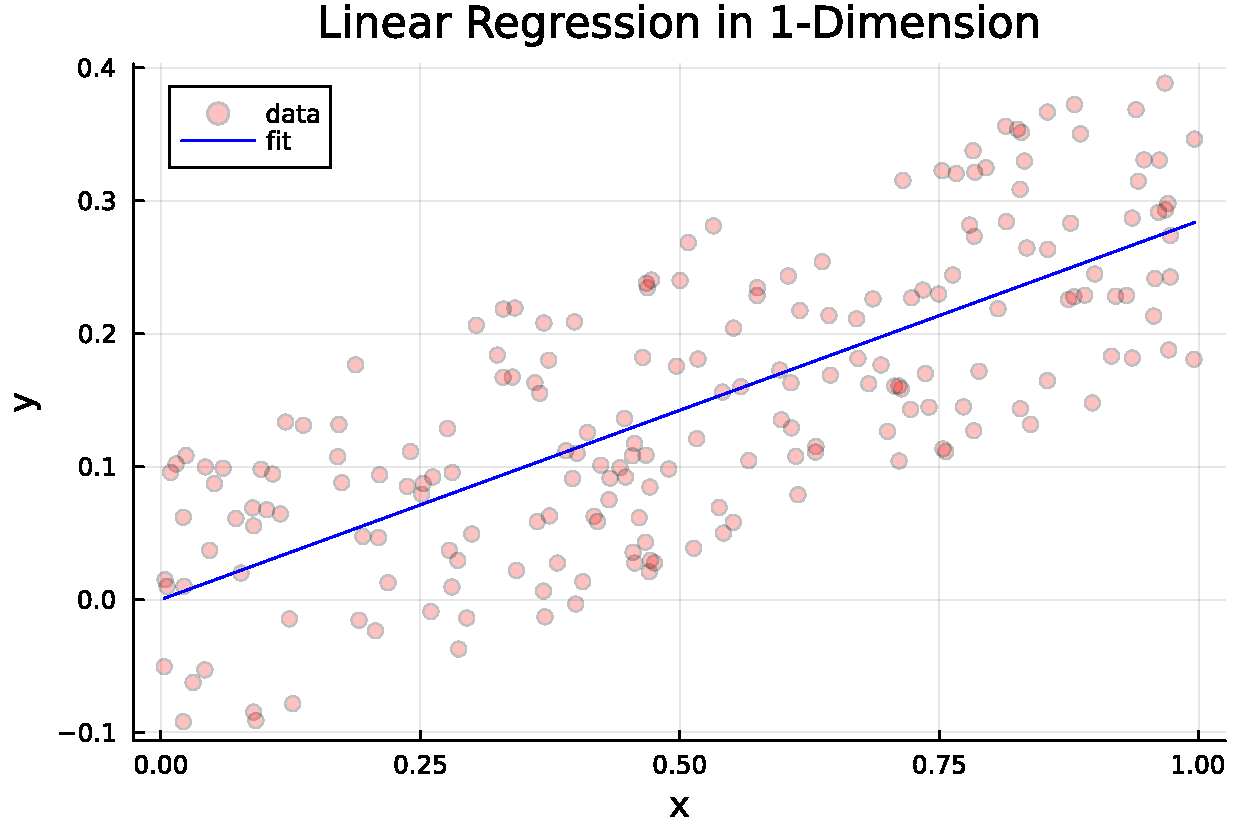
\includegraphics[width=0.9\columnwidth]{ml-figures/gpr/linear-regression.pdf}
  \end{centering}
  \caption{A standard linear regression fit on some noisy data.}
\end{figure}
We can also fit a y-intercept (aka \textit{bias}) by augmenting the design matrix $X$ to contain an extra row with all $1$'s, i.e.
\begin{equation}
  X[D+1, :] = (1, ..., 1)
\end{equation}

Standard linear regression assumes that our data, $\mathcal{D}$, are perfect, but we can clearly see that the above data are noisy. To account for this, we need to make our model \textit{Bayesian} by augmenting it to consider the measurement error. We define
\begin{align}
    f(\mathbf{x}) &= \mathbf{x}^T\mathbf{w} \\
    \mathbf{y} &= f(\mathbf{x}) + \mathbf{\epsilon} \\
    \mathbf{\epsilon} &\sim \mathcal{N}(0, \sigma_n^2)
\end{align}

or, in words, our observed values differ from the \textit{truth} by identically, independently, distributed Gaussian noise with mean $0$ and variance $\sigma_n^2$. The assumption that the noise is i.i.d. is critical because it allows us to simplify the \textit{likelihood} function by separating out each individual contribution by our datapoints:

\begin{align}
    p(\mathbf{y}\vert X,\mathbf{w}) &:= \prod\limits_i^n p(\mathbf{y}_i \vert \mathbf{x}_i, \mathbf{w}) \\
    &= \prod\limits_i^n \frac{1}{\sqrt{2\pi\sigma_n^2}}\exp\left( -\dfrac{(\mathbf{y}_i-\mathbf{x}_i^T\mathbf{w})^2}{2\sigma_n^2}\right)\\
    &= \dfrac{1}{(2\pi\sigma_n^2)^{n/2}}\exp\left( -\frac{1}{2\sigma_n^2}\lvert \mathbf{y} - X^T\mathbf{w}\rvert^2 \right) \\
    &= \mathcal{N}\left(X^T\mathbf{w}, \sigma_n^2I\right)
\end{align}

To perform inference with this updated model, we apply Baye's Rule, that is:


\begin{equation}
  p(\mathbf{w}\vert \mathbf{y}, X) = \dfrac{p(\mathbf{y}\vert X, \mathbf{w})p(\mathbf{w})}{p(\mathbf{y}\vert X)}
\end{equation}
where
\begin{itemize}[noitemsep, nolistsep]
\item $p(\mathbf{w}\vert \mathbf{y}, X)$ is the \textit{posterior distribution}
\item $p(\mathbf{y}\vert X, \mathbf{w})$ is the \textit{likelihood}
\item $p(\mathbf{w})$ is the \textit{prior distribution}
\item $p(\mathbf{y} \vert X)$ is the \textit{marginal likelihood}, i.e. the normalization constant
\end{itemize}
It is now that the utility of choosing gaussian distributions for our likelihood and prior becomes clear. We have
\begin{align}
  p(\mathbf{w}\vert\mathbf{y},X) &\propto \exp\left(-\frac{1}{2\sigma_n^2}(\mathbf{y}-X^T\mathbf{w})^T(\mathbf{y}-X^T\mathbf{w}) \right)\exp\left(-\frac{1}{2}\mathbf{w}^T\Sigma_p^{-1}\mathbf{w}\right)
\end{align}
Taking the log and expanding leads to
\begin{align}
  \log(p(\mathbf{w}\vert \mathbf{y}, X))&= \frac{1}{2}\left[ \frac{1}{\sigma_n^2}\mathbf{y}^T\mathbf{y} - \frac{1}{\sigma_n^2}\mathbf{y}^TX^T\mathbf{w} - \frac{1}{\sigma_n^2}\mathbf{w}^TX\mathbf{y} + \frac{1}{\sigma_n^2}\mathbf{w}^TXX^T\mathbf{w} + \mathbf{w}^T\Sigma_p^{-1}\mathbf{w}\right] \\
  &= \frac{1}{2}\left[ \mathbf{w}^T\left(\frac{1}{\sigma_n^2}XX^T+\Sigma_p^{-1}\right)\mathbf{w} -\left(\frac{1}{\sigma_n^2}\mathbf{y}^TX^T\right)\mathbf{w} - \mathbf{w}^T\left(\frac{1}{\sigma_n^2}X\mathbf{y}\right)  + \mathbf{y}^T\frac{1}{\sigma_n^2}\mathbf{y}\right]\\
  &= \mathbf{w}^TA\mathbf{w} - B^T\mathbf{w} - \mathbf{w}^TB + C
\end{align}
where we have defined
\begin{align}
    A &:= \frac{1}{\sigma_n^2}XX^T + \Sigma_p^{-1} \\
    B &:= \frac{1}{\sigma_n^2}X\mathbf{y} \\
    C &:= \mathbf{y}^T\frac{1}{\sigma_n^2}\mathbf{y}
\end{align}
Now we can complete the square so that
\begin{equation}
    \mathbf{w}^TA\mathbf{w} - B^T\mathbf{w} - \mathbf{w}^TB + C = \left(\mathbf{w} - \bar{\mathbf{w}} \right)^TA\left(\mathbf{w} - \bar{\mathbf{w}} \right) + K
    \end{equation}
    leading to 
    \begin{align}
    \bar{\mathbf{w}} &= A^{-1}B = \frac{1}{\sigma_n^2}\left(\frac{1}{\sigma_n^2}XX^T + \Sigma_p^{-1}\right)^{-1}X\mathbf{y} \\
    K &= C- \bar{\mathbf{w}}^TA\bar{\mathbf{w}}
\end{align}
Since $K$ does not depend on $\mathbf{w}$ directly, it may be absorbed into the normalization of $p(\mathbf{w}\vert \mathbf{y}, X)$. Thus we are left with
\begin{align}
    p(\mathbf{w}\vert\mathbf{y},X) &= \mathcal{N}\left( \bar{\mathbf{w}}=\frac{1}{\sigma_n^2}A^{-1}X\mathbf{y}, \Sigma=A^{-1}\right) \\
    A &= \frac{1}{\sigma_n^2}XX^T+\Sigma_p^{-1}
\end{align}
This result gives us the gaussian distriubtion over the space of possible parameter vectors $\mathbf{w}$. To use this distribution to make predictions, consider a newly supplied testpoint $\mathbf{x}_*$. We want to find
\begin{equation}
    p(y_* \vert \mathbf{x}_*, \mathbf{y}, X)
\end{equation}
We do this by marginalizing over our weight distribution, i.e.
\begin{equation}
    p(y_* \vert \mathbf{x}_*, \mathbf{y}, X) = \int_{\mathbf{w}} p(y_*\vert \mathbf{x}_*,\mathbf{w})p(\mathbf{w}\vert \mathbf{y}, X)d\mathbf{w}
\end{equation}
If we make the further assumption that testing points are i.i.d. guassian distriubted, we see that this integral is the product of two gaussians and therefore is also a guassian. To find the mean and covariance of the predictive distribution, we check
\begin{align} 
    \bar{y}_* &= \mathbb{E}[y_*] = \mathbb{E}[\mathbf{x}_*^T\mathbf{w}] = \mathbf{x}_*^T\mathbb{E}[\mathbf{w}] = \mathbf{x}_*^T\bar{\mathbf{w}} \\
    \text{Cov}(y_*) &= \mathbb{E}[(y_*-\bar{y}_*)(y_*-\bar{y}_*)^T] \\
    &= \mathbb{E}[(\mathbf{x}_*^T\mathbf{w}-\mathbf{x}_*^T\bar{\mathbf{w}})(\mathbf{x}_*^T\mathbf{w}-\mathbf{x}_*^T\bar{\mathbf{w}})^T] \\
    &= \mathbb{E}[\mathbf{x}_*^T(\mathbf{w}-\bar{\mathbf{w}})(\mathbf{w}-\bar{\mathbf{w}})^T\mathbf{x}_*] \\
    &= \mathbf{x}_*^T\mathbb{E}[(\mathbf{w}-\bar{\mathbf{w}})(\mathbf{w}-\bar{\mathbf{w}})^T]\mathbf{x}_* \\
    &= \mathbf{x}_*^T\text{Cov}(\mathbf{w})\mathbf{x}_* \\
    &= \mathbf{x}_*^TA^{-1}\mathbf{x}_*
\end{align}
so that
\begin{equation}
    \boxed{p(y_* \vert \mathbf{x}_*, \mathbf{y}, X) = \mathcal{N}\left(\mathbf{x}_*^T\mathbf{w},\;  \mathbf{x}_*^TA^{-1}\mathbf{x}_*\right)}
\end{equation}


Let's now take a break from our Bayesian regression discussion and return to the standard linear regression model for a moment. The key drawback of linear models like this is, of course, that they're \textit{linear}! Considering that many (most) \textit{interesting} relationships are non-linear, how can we extend our simple linear model to enable us to perform complicated non-linear fits?

In the parlance of machine learning, the simple solution is to do \href{https://en.wikipedia.org/wiki/Feature_engineering}{feature engineering}. If our inital feature vector is
\begin{equation}
    \mathbf{x} = (x_1, ..., x_n)
\end{equation}
we can use our \textit{expertise} to concoct new combinations of these features to produce the agumented vector
\begin{equation}
    \tilde{\mathbf{x}} = (x_1, ..., x_n, x_1^2, \;sin(x_2), \;x_5x_7/x_4,\;...)
\end{equation}

As an example, a linear classifier is unable to distinguish points inside a circle from those outside just from the $(x,y)$ coordinates alone. Augmenting the feature vector to include the squared radius $x^2+y^2$ as a new feature removes this obstacle. This works because the \textit{linear} part of linear regression only refers to the fact that our model takes \textit{linear combinations} of feature variables to produce it's output. There is no restriction that the features themselves need to be independent variables! This same idea is what makes methods like \href{https://www.pnas.org/doi/10.1073/pnas.1517384113}{SINDy} work which use libraries of polynomial combinations of base features.

Constructing new features is often more art than science. To standardize the process, let's abstract the mapping from the original feature vector $\mathbf{x}$ to the augmented vector $\tilde{\mathbf{x}}$. This is accomplished via the projection map $\phi:\mathbb{R}^D \to \mathbb{R}^N$ where
\begin{equation}
    \mathbf{x} \mapsto \tilde{\mathbf{x}} = \phi(\mathbf{x})
\end{equation}
The result is that our linear model updates to become
\begin{equation}
    f(\mathbf{x}) := \phi(\mathbf{x})^T\mathbf{w}
\end{equation}
where the weight vector has gone from $D$ dimensional to $N$ dimensional. Similarly, the normal equations for $\mathbf{w}$ update to become
\begin{equation}
    \mathbf{w} = (\Phi\Phi^T)^{-1}\Phi\mathbf{y}
\end{equation}
where $\Phi = \phi(X)$ is the $N\times n$ matrix resulting from applying $\phi$ columnwise to $X$.

The following example shows how to use such a mapping to produce a quadratic polynomial fit.

\begin{figure}[h]
  \begin{centering}
    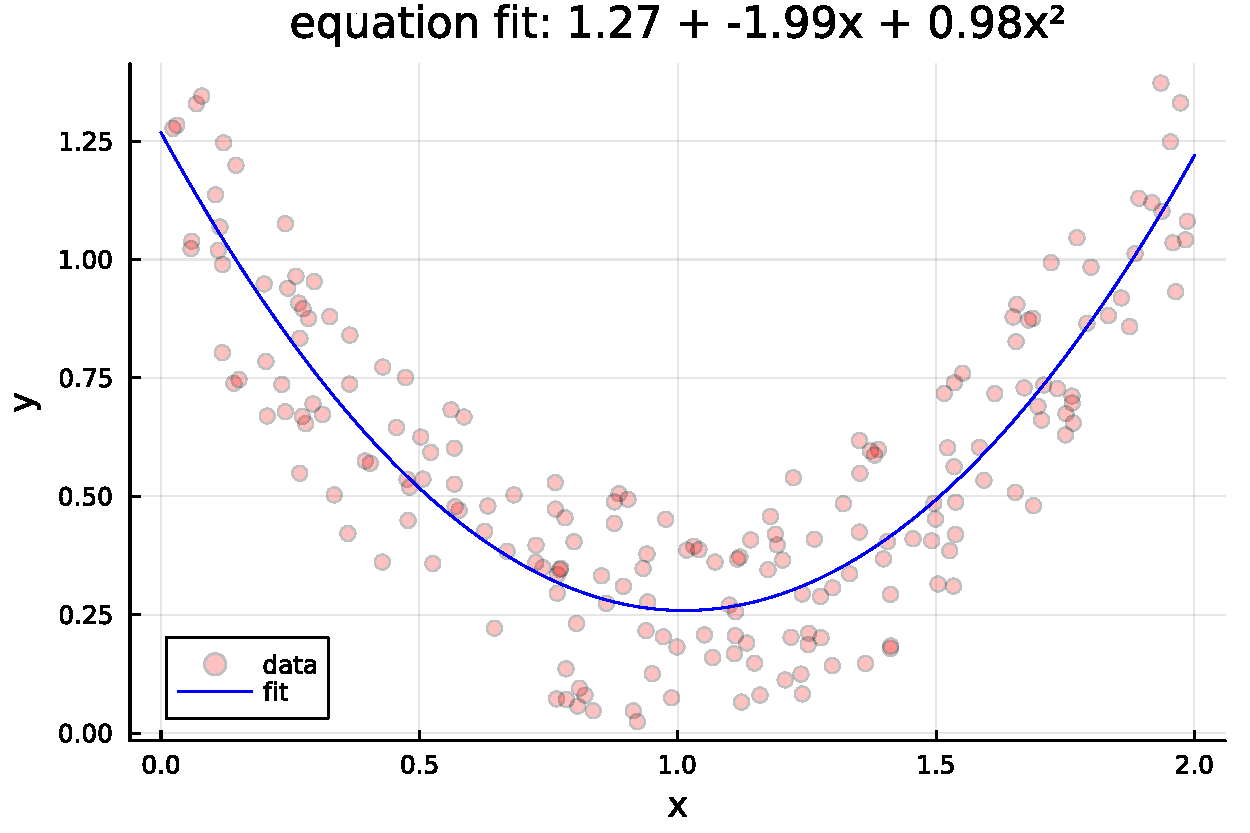
\includegraphics[width=0.85\columnwidth]{ml-figures/gpr/polynomial-regression.pdf}
  \end{centering}
  \caption{An example of polynomial regression for which we fit a quadratic polynomial to some noisy data.}
  \label{fig:polynomial-regression}
\end{figure}
We see from Figure \ref{fig:polynomial-regression} that our linear regression model found a great fit for a 2nd order polynomial when supplied with polynomial features. Let's update our Bayesian regression scheme to reflect the use of our feature projection map $\phi$. First we define
\begin{align}
  \Phi &:= \phi(X) \\
  \phi_* &:= \phi(\mathbf{x}_*)
\end{align}

Our predictive distribution therefore becomes
\begin{align}
  p(y_* \vert \mathbf{x}_*, X, \mathbf{y}) &= \mathcal{N}\left(\frac{1}{\sigma_n^2}\phi_*^TA^{-1}\Phi\mathbf{y}, \;\phi_*^TA^{-1}\phi_*\right) \\
  A &= \frac{1}{\sigma_n^2}\Phi\Phi^T + \Sigma_p^{-1}
\end{align}
Great! Now we can do our Bayesian inference with non-linear features given by $\phi$. There is a \textit{massive} problem with this approach, however. Our order 2 polynomial map $\phi$ takes us from a $D$ dimenional feature vector to $(D+1)!$ many. This means that as we add more features to our feature map, the dimension of the resulting vector will quickly become prohibitively large. Looking at our current model equations, we see that the bottleneck is the matrix inversion of $A$ which requires we invert an $N\times N$ matrix. Our prediction (i.e. the mean) involves multiplication on the right by the $n$ dimensional vector $\mathbf{y}$. With that in mind, perhaps we can reformulate the above into an equivalent form using at most an $n\times n$ dimensional matrix.

Let $K:= \Phi^T\Sigma_p\Phi$. Observe the following:
\begin{align}
  \frac{1}{\sigma_n^2}\Phi(K+\sigma_n^2I) &= \frac{1}{\sigma_n^2}\Phi\left(\Phi^T\Sigma_p\Phi + \sigma_n^2I \right) \\
  &= \frac{1}{\sigma_n^2}\Phi\Phi^T\Sigma_p\Phi + \Phi I \\
  &= \left(\frac{1}{\sigma_n^2}\Phi\Phi^T \right)\Sigma_p\Phi + \left(\Phi I \Phi^{-1}\Sigma_p^{-1} \right)\Sigma_p\Phi \\
  &= \left(\frac{1}{\sigma_n^2}\Phi\Phi^T + \Sigma_p^{-1}\right)\Sigma_p\Phi \\
  &= A\Sigma_p\Phi
\end{align}

From there we see that
\begin{align}
    A^{-1}\frac{1}{\sigma_n^2}\Phi\left(K+\sigma_n^2I\right) &= \Sigma_p\Phi \\
    \Rightarrow \frac{1}{\sigma_n^2}A^{-1}\Phi &= \Sigma_p\Phi\left(K + \sigma_n^2I\right)^{-1} \\
    \Rightarrow \frac{1}{\sigma_n^2}\phi_*^TA^{-1}\Phi &= \phi_*^T\Sigma_p\Phi\left(K + \sigma_n^2I\right)^{-1}
\end{align}
For the covariance, we utilize the matrix inversion lemma \textcolor{red}{(ADD REFERENCE HERE)} which states
\begin{equation}
    (Z + UWV^T)^{-1} = Z^{-1} - Z^{-1}U(W^{-1} + V^TZ^{-1}U)^{-1}V^TZ^{-1}
\end{equation}
With the identification
\begin{align}
    Z^{-1} &\to \Sigma_p \\
    W^{-1} &\to \sigma_n^2I \\
    V &\to \Phi \\
    U &\to \Phi
\end{align}
we find
\begin{align}
    \Sigma_p - \Sigma_p\Phi\left(\Sigma_p + \Phi^T\Sigma_p\Phi \right)^{-1}\Phi^T\Sigma_p  &= \left(\Sigma_p^{-1} + \Phi\frac{1}{\sigma_n^2}I\Phi^T\right)^{-1}\\
    &= \left(\frac{1}{\sigma_n^2}\Phi\Phi^T + \Sigma_p^{-1}\right)^{-1}  \\
    &= A^{-1}
\end{align}
Thus, we have the equivalent form for our predictive distribution:
\begin{equation}
    \boxed{p(y_*\vert \mathbf{x}_*, X, \mathbf{y}) =\\ \mathcal{N}\left( \phi_*^T\Sigma_p\Phi(K+\sigma_n^2I)^{-1}\mathbf{y}, \; \phi_*^T\Sigma_p\phi_* - \phi_*^T\Sigma_p\Phi(K+\sigma_n^2I)^{-1}\Phi^T\Sigma_p\phi_*\right)}
\end{equation}
where the pesky $N\times N$ term has been replaced by the $n\times n$ matrix $\Phi^T\Sigma_p\Phi$.


We now make the the \textit{key} observation that the only matrices that appear in the above expression are
\begin{align}
    &\Phi^T\Sigma_p\Phi, &\phi_*^T\Sigma_p\phi_* \\
    &\phi_*^T\Sigma_p\Phi, &\Phi^T\Sigma_p\phi_*
\end{align}
whose matrix elements we can write abstractly as
\begin{equation}
    \phi(\mathbf{x})^T\Sigma_p\phi(\mathbf{x}')
\end{equation}

To fit our model, we must determine appropriate values for the symmetric, positive semi-definite covariance matrix $\Sigma_p$ (and $\sigma_n$ too, technically). Instead, we observe that this matrix product is a quadratic form which we can think of as representing an inner product on our transformed vectors:
\begin{equation}
    K_{ij} = k(\mathbf{x}_i, \mathbf{x}_j) = \langle \phi(\mathbf{x}_i), \phi(\mathbf{x}_j)\rangle
\end{equation}
We call the function $k(\mathbf{x},\mathbf{x}')$ the \textit{kernel function} or the \textit{covariance function}.

All we need to perform the above calculations are the matrix elements of K applied to our data $\mathcal{D}$ and any test points $\mathbf{x}_*$ we wish to apply our model to. In effect, this means we are free to use feature vectors \href{https://www.youtube.com/watch?v=XUj5JbQihlU&t=25m53s}{of any dimension, including $\infty$}. The idea here is that the kernel function represents an inner product over \textit{some} vector space. As it turns out, the RBF kernel corresponds to a an \href{https://math.stackexchange.com/questions/276707/why-does-a-radial-basis-function-kernel-imply-an-infinite-dimension-map}{infinite dimensional feature vector}.

There are many choices for the kernel function. One of the most popular is the RBF (radial basis function) kernel, also commonly referred to as the \textit{squared exponential kernel}:
\begin{equation}
    k_{\text{rbf}}(\mathbf{x}, \mathbf{x}') := \sigma_f^2\exp(-\frac{1}{2\ell^2}\lvert \mathbf{x}-\mathbf{x}'\rvert^2)
\end{equation}

where $\sigma_f^2$ is the *signal variance* and $\ell$ denotes the similarity length scale.

For notational convenience, let's define
\begin{align}
    K &:= k(X,X) \\
    K_{**} &:= k(X_*, X_*) \\
    K_{*} &:= k(X, X_*)
\end{align}

then, our predictive distribution takes the final, \textit{clean} form
\begin{equation}
    \boxed{p(\mathbf{y}_* \vert X_*, X, \mathbf{y}) = \mathcal{N}\left( K_*^T(K+\sigma_n^2I)^{-1}\mathbf{y},\; K_{**}-K_{*}^T(K+\sigma_n^2I)^{-1}K_*\right)}
\end{equation}
This is the \textit{end-result} of Gaussian Process Regression acheived via the \textit{weight-space view}.


\subsubsection{The Function-space View}

So far our approach has been to generalize the standard linear regression model to allow for fitting over a (possibly infinite) basis of features with consideration for measurement and model uncertainty (our Bayesian priors). In essence, the idea was to fit the distribution of all possible weights conditioned on the available training data, $p(\mathbf{w} \vert X, \mathbf{y})$. A second \textit{equivalent} approach is to instead consider the distribution of all possible model function $f(\mathbf{x})$. By constructing a Bayesian prior over this space, we constrain the space of possible model functions and learn a \textit{distribution} over all allowed model functions, $p(f \vert X, \mathbf{y})$. To do so we will need to develop the abstract machinery of distributions over function spaces. When these distributions are Gaussian, the result is called a \textbf{Gaussian process}.

By this point, we are very familiar with the Gaussian distribution, a.k.a. the Normal distribtion $\mathcal{N}(\mu, \sigma^2)$. This distribution is defined by a mean value $\mu$ and a variance $\sigma^2$. It's \textit{big brother} is the \textbf{Multivariate Normal Distribution}, $\mathcal{N}(\mathbf{\mu}, \Sigma)$, described be a vector of means $\mathbf{\mu}$ and a covariance matrix $\Sigma$. A natural question, then, is can we generalize the concept of the Gaussian distribution from $N$ dimensions to being defined over a continuous field? This leads us naturally to the development of a so-called \textbf{Gaussian Process}.\\

\fbox{
  \parbox{0.8\columnwidth}{
    \noindent\textbf{Definition}: A \textit{Gaussian Process}, $\mathcal{GP}$, is a collection of random variables for which any finite subset are described by a joint Gaussian distribution.
  }
}\\


To see where this comes from, recall that in our previous derivation, we already made the assumption that all our our data points $\mathcal{D}$ are i.i.d. Gaussian distributed. A gaussian process is the natural extension of this and makes the assumption that the continuous set from which are data are sampled are so Guassian that any finite sample will be jointly Gaussian distributed. The term process is used to distinguish between finite collections of random variables (distributions) and their continuous counterparts described here.

Because each finite subset of this continuous collection is jointly gaussian, we can completely specify a Gaussian Process with two functions: the mean function $m(\mathcal{x})$ and the covariance function $k(\mathbf{x},\mathbf{x}')$. To denote this, we typically write
\begin{equation}
    f(\mathbf{x}) \sim \mathcal{GP}(m(\mathbf{x}), k(\mathbf{x},\mathbf{x}'))
\end{equation}

To see this in action, recall our Bayesian regression model
\begin{equation}
  f(\mathbf{x} = \phi(\mathbf{x})^T\mathbf{w} \qquad \mathbf{w}\sim\mathcal{N}(\mathbf{0}, \Sigma_p)
\end{equation}
where we have set the prior on $\mathcal{w}$ to have zero mean. The mean function is given by the expectation value of our model:
\begin{equation}
  \mathbb{E}[f(\mathbf{x})] = \phi(\mathbf{x})^T\mathbb{E}[\mathbf{w}] = 0
\end{equation}
and the covariance function is given by
\begin{equation}
  \mathbb{E}[f(\mathbf{x})f(\mathbf{x'})] = \phi(\mathbf{x})^T\mathbb{E}[\mathbf{w}\mathbf{w}^T]\phi(\mathbf{x}') = \phi(\mathbf{x})^T\Sigma_p\phi(\mathbf{x}')
\end{equation}

To repeat the point, the key feature of Gaussian processes is that finite subsets are jointly Gaussian distributed. Thus we can we can split our data into the testpoints $\mathcal{D}=(X,\mathbf{y})$ and testpoints $X_*$ t and treat each collection as joint distributions with the following priors:
\begin{equation}
  \begin{bmatrix} \mathbf{f} \\ \mathbf{f}_* \end{bmatrix} \sim \mathcal{N}\left(\mathbf{0},\begin{bmatrix} K(X,X) & K(X,X_*) \\ K(X_*,X) & K(X_*,X_*) \end{bmatrix}\right)
\end{equation}
where $\mathbf{f}:= f(X)$ and $\mathbf{f}_* = f(X_*)$.

To obtain our predictive distribution, $p(\mathbf{f}_* \vert X_*, X, \mathbf{y})$, we \textit{condition the joint prior distribution} on the observations. To see how this works, consider a general joint gaussian distribution given by
\begin{equation}
\begin{bmatrix} x \\ y \end{bmatrix} \sim \mathcal{N}\left( \begin{bmatrix}\mu_x \\ \mu_y\end{bmatrix},\; \begin{bmatrix} \Sigma_{xx} & \Sigma_{xy} \\ \Sigma_{yx} & \Sigma_{yy} \end{bmatrix}\right)
\end{equation}

define the centered values $\tilde{x} := x-\mu_x$ and $\tilde{y} := x-\mu_y$. Define the intermediate variable
\begin{equation}
    z := \tilde{x} - A\tilde{y}
\end{equation}
Note that since we've subtracted out the mean we have $\mathbb{E}[\tilde{x}] = \mathbb{E}[\tilde{y}] = \mathbb{E}[z] = 0$. Let's now find $A$.
\begin{align}
    \mathbb{E}[z\tilde{y}^T] &= \mathbb{E}[(\tilde{x}-A\tilde{y})\tilde{y}^T] \\
    &= \mathbb{E}[\tilde{x}\tilde{y}^T - A\tilde{y}\tilde{y}] \\
    &= \mathbb{E}[\tilde{x}\tilde{y}^T] - \mathbb{E}[A\tilde{y}\tilde{y}^T] \\
    &= \Sigma_{xy} - A\mathbb{E}[\tilde{y}\tilde{y}^T] \\
    &= \Sigma_{xy} - A\Sigma_{yy}
\end{align}
Therefore if we choose $A$ so that $z$ and $\tilde{y}$ are independent and uncorrelated, then $\Sigma_{zy} = \mathbb{E}[z\tilde{y}^T] = 0$. Using this assumption, we find
\begin{equation}
    0 = \mathbb{E}[z\tilde{y}^T] = \Sigma_{xy}-A\Sigma_{yy} \\ \Rightarrow \boxed{A = \Sigma_{xy}\Sigma_{yy}^{-1}}
\end{equation}
If we now condition $\tilde{x}$ on $\tilde{y}$ (i.e. look at $\tilde{x}$ when $\tilde{y}$ is constant), we find
\begin{align}
    \mathbb{E}[\tilde{x}\vert\tilde{y}] &= A\tilde{y} + \mathbb{E}[z] \\
    &= A\tilde{y} + 0 \\
    &= \Sigma_{xy}\Sigma_{yy}^{-1} \\
\end{align}
By manipulating this expression, we can now derive $\mathbb{E}[x\vert y]$ as follows:
\begin{align}
    \mathbb{E}[x\vert\tilde{y}] &= \mathbb{E}[\tilde{x}\vert\tilde{y}] + \mu_x \\
    &= \mu_x + \Sigma_{xy}\Sigma_{yy}^{-1}\tilde{y} \\
\end{align}
\begin{equation}
\boxed{\mathbb{E}[x\vert y] = \mu_x + \Sigma_{xy}\Sigma_{yy}^{-1}(y-\mu_y)}
\end{equation}

Similarly for the covariance, we have
\begin{align}
    \text{Cov}(x \vert y) &= \text{Cov}(\tilde{x}+\mu_x \vert \tilde{y}) \\
    &= \text{Cov}(\tilde{x}+\mu_x \vert \tilde{y} + \mu_y) \\
    &= \text{Cov}(\tilde{x}\vert(\tilde{y}+\mu_y)) \\
    &= \text{Cov}(\tilde{x}\vert \tilde{y}) \\
    &= \text{Cov}((z+A\tilde{y})\vert\tilde{y}) \\
    &= \text{Cov}(z) + {A\text{Cov}(\tilde{y})} \\
    &= \text{Cov}(z) + 0 \\
    &= \mathbb{E}[zz^T] \\
    &= \mathbb{E}[(\tilde{x}-A\tilde{y})(\tilde{x}-A\tilde{y})^T]\\
    &= \mathbb{E}[\tilde{x}\tilde{x}^T - A\tilde{y}\tilde{x}^T -x(A\tilde{y})^T + A\tilde{y}\tilde{y}^TA^T] \\
    &= \Sigma_{xx} - A\Sigma_{yx} - \Sigma_{xy}A^T + A\Sigma_{yy}A^T \\
    &= \Sigma_{xx}-(\Sigma_{xy}\Sigma_{yy}^{-1})\Sigma_{yx} - \Sigma_{xy}(\Sigma_{yy}^{-1})^T\Sigma_{xy}^T + \Sigma_{xy}\Sigma_y^{-1}\Sigma_{y}(\Sigma_{y}^{-1})^T\Sigma_{xy}^T \\
    &= \Sigma_{xx} - \Sigma_{xy}\Sigma{yy}^{-1}\Sigma_{xy}^T - \Sigma_{xy}(\Sigma_{yy}^{-1})^T\Sigma_{xy}^T + \Sigma_{xy}(\Sigma_{yy}^{-1})^T\Sigma_{xy}^T \\
    &= \Sigma_{xx}-\Sigma_{xy}\left[\Sigma_{yy}^{-1} - (\Sigma_{yy}^{-1})^T + (\Sigma_{yy}^{-1})^T \right]\Sigma_{xy}^T \\
    &= \Sigma_{xx} - \Sigma_{xy}\Sigma_{yy}^{-1}\Sigma_{yx}
\end{align}

\begin{equation}
\boxed{\text{Cov}(x \vert y) = \Sigma_{xx} - \Sigma_{xy}\Sigma_{yy}^{-1}\Sigma_{yx}}
\end{equation}
Armed with this identity for joint Guassian distributions, we are ready to derive the predictive distribution for Gaussian Process Regression. We find:
\begin{equation}
  p(\mathbf{f}_* \vert X_*, X, \mathbf{y} = \mathcal{N}\left( K_*^TK^{-1}\mathbf{f},\; K_{**}-K_*^TK^{-1}K_*\right).
\end{equation}
To account for noisy observations, we can augment our correlation function to include a noise offset. The joint distrubtion then becomes:
\begin{equation}
  \begin{bmatrix} \mathbf{f} \\ \mathbf{f}_* \end{bmatrix} \sim \mathcal{N}\left(\mathbf{0},\begin{bmatrix} K(X,X)-\sigma_n^2I & K(X,X_*) \\ K(X_*,X) & K(X_*,X_*) \end{bmatrix}\right)
\end{equation}
which leads to the predictive distribution
\begin{equation}
  \boxed{p(\mathbf{f}_* \vert X_*, X, \mathbf{y}) = \mathcal{N}\left( K_*^T\left[K + \sigma_n^2 I\right]^{-1}\mathbf{f},\; K_{**}-K_*^T\left[K + \sigma_n^2 I\right]^{-1}K_*\right)}
\end{equation}


\subsubsection{Doing it in Julia}

To see how we can use this in practice, let's first construct some sample data which we seek to model as a Gaussian Process
\begin{figure}[h]
  \begin{centering}
    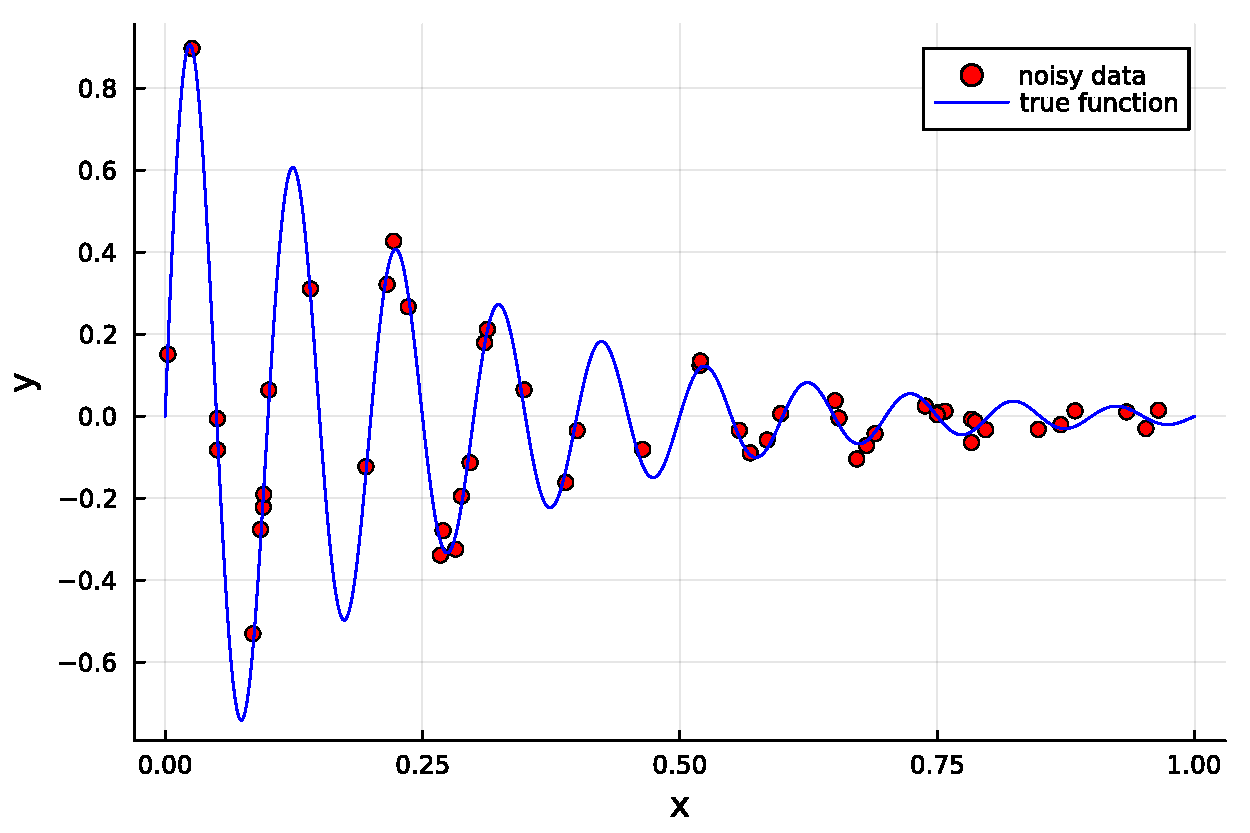
\includegraphics[width=0.8\columnwidth]{ml-figures/gpr/training-data.pdf}
  \end{centering}
\end{figure}

The excellent package \href{https://juliagaussianprocesses.github.io/KernelFunctions.jl/dev/userguide/}{KernelFunctions.jl} provides a clean interface to create various kernel functions and apply them to data to create our $K$-matrices. Due to the fact that kernel functions obey composition laws, we can easily build up complicated Kernels from basic pieces via function composition with $\circ$

\begin{figure}
  \centering
  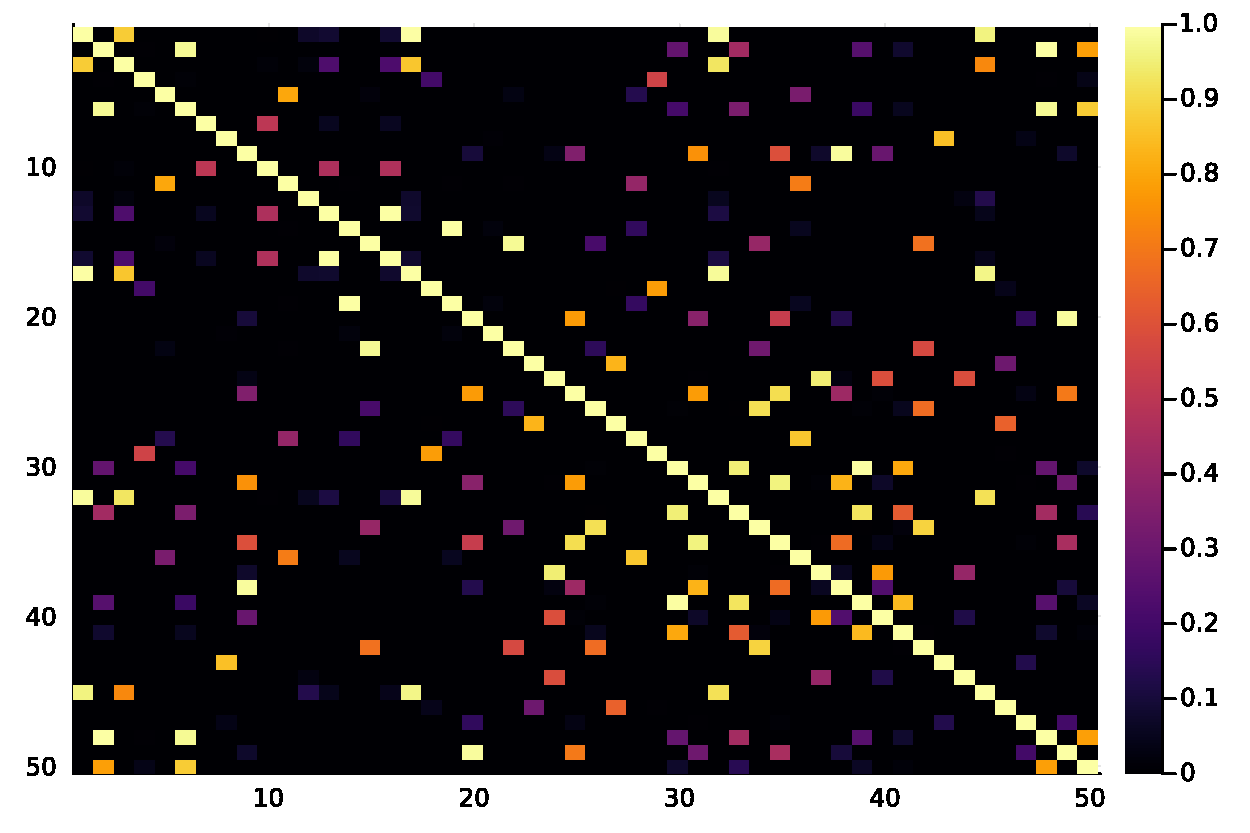
\includegraphics[width=0.8\columnwidth]{ml-figures/gpr/kernel-matrix.pdf}
\end{figure}
Unsurprisingly, there is a lot of activation on the diagonal as for a single datapoint $\mathbf{x}$, we have
\begin{equation}
    k(\mathbf{x},\mathbf{x}) = \exp\left(-\frac{0}{2\ell^2} \right) = 1.0
\end{equation}

The package \href{https://juliagaussianprocesses.github.io/AbstractGPs.jl/dev/}{AbstractGPs.jl} provides an excellent way to define Gaussian Processes by supplying mean and kernel functions. We can then sample from our GPs with a simple interface designed to extend the basic functions from \texttt{Statistics.jl}. From an \texttt{AbstractGP} we can construct a \texttt{FiniteGP} by \textit{indexing} into our datasets. The procedure can be summarized as follows
\begin{enumerate}
\item Build a kernel function $k(\cdot, \cdot)$ via composition using \texttt{KernelFunctions.jl}
\item Construct an a Gaussian Process $f\sim\mathcal{GP}$ abstractly using \texttt{AbstractGPs.jl}
\item Construct a finite representation of our GP, $f_x$, over our training data
\item Construct a posterior Gaussian Process from $f_x$ and our training targets $\mathbf{y}$.
\item Construct a finite representation of the posterior GP applied to our prediction data
\item Sample this final distribution to obatin a prediction via \texttt{mean()} and variances via \texttt{var()}. Alternatively, we can obtain a multivariate normal distribution for each point by calling \texttt{marginals()}.
\end{enumerate}

\begin{figure}[h]
  \centering
  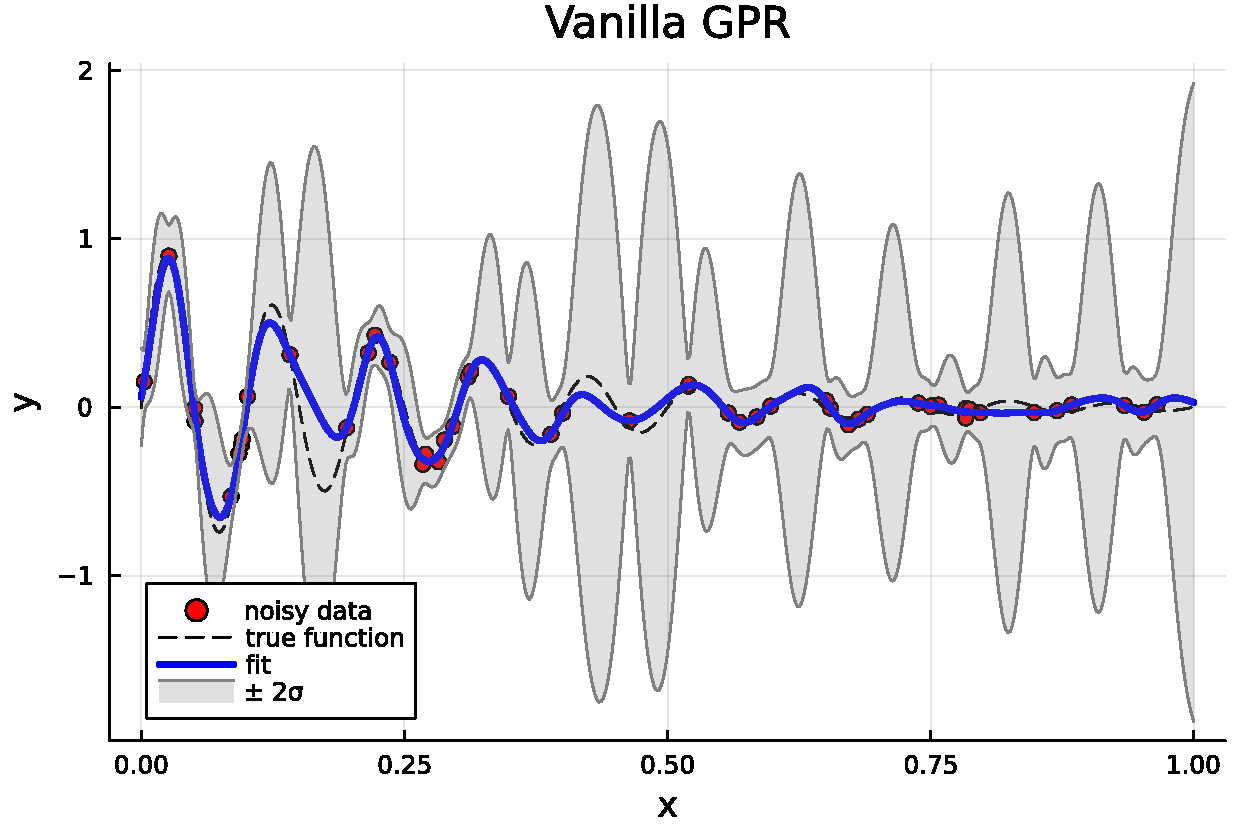
\includegraphics[width=0.85\columnwidth]{ml-figures/gpr/vanilla-gpr.pdf}
  \caption{A Gaussian Process fit to the training data illustrating the predication (means) and a $\pm 2\sigma$ uncertainty interval. We can clearly see how the uncertainty is larger for inputs far away from supplied training data.}
  \label{fig:vanilla-gpr}
\end{figure}

\subsubsection{Fitting the Kernel Hyperparameters}
At this point, it is easy to think we are finished; we \textit{already} fit the Guassian process. However, we were forced to choose values for both $\ell$ and $\sigma^2$ kernel parameters. How can we optimally select the ideal hyperparameters for our Gaussian Process? This question leads us into the realm of \href{https://gaussianprocess.org/gpml/chapters/RW5.pdf}{Bayesian Model Selection}. Rather than focusing specifically on our Gaussian Process model, let's take a step back and think about the process of model selection from a Bayesian perspective.

There are several levels of parameters in machine learning. At the lowest level, we have the model weights $\mathbf{w}$. Above that, we have model hyperparameters, $\theta$. At the top we have model structure $\mathcal{H}$. In our Bayesian framework, we can consider prior distributions defined at each of these levels which codify credences for how much we trust a particular model, hyperparameter, etc. At the bottom, we have
\begin{equation}
  p(\mathbf{w} \vert X, \mathbf{y}, \theta, \mathcal{H}_i) = \frac{p(\mathbf{y} \vert X, \mathbf{w}, \theta, \mathcal{H}_i) p(\mathbf{w}\vert \theta, \mathcal{H}_i) }{p(\mathbf{y}\vert X, \theta, \mathcal{H}_i)}
\end{equation}

If this looks confusing, consider Bayes rule for 3 events $R, H, S$. We have:
\begin{align}
  P(R \vert H, S) &= \frac{P(R,H,S)}{P(H,S)} \\
  &= \frac{P(H \vert R, S)P(R, S)}{P(H,S)}\\
  &= \frac{P(H \vert R, S)P(R\vert S)P(S)}{P(H\vert S)P(S)} \\
  &= \frac{P(H \vert R, S)P(R\vert S)}{P(H\vert S)}
\end{align}
To get the result, just think of $\theta$ and $\mathcal{H}_i$ as a single \textit{event} and translate the above to distribution functions. % See \href{https://math.stackexchange.com/questions/1281454/bayes-rule-with-3-variables}{stack exchange link}.

The prior $p(\mathbf{w}\vert \theta, \mathcal{H}_i)$ encodes any knowledge we have about the parameters prior to seeing the data. The denominator is the \textit{marginal likelihood} and is given by
\begin{equation}
    p(\mathbf{y}\vert X, \theta, \mathcal{H}_i) = \int d\mathbf{w}\; p(\mathbf{y} \vert X, \mathbf{w}, \theta, \mathcal{H}_i)p(\mathbf{w}\vert \theta, \mathcal{H}_i)
\end{equation}
The next level up is to express the distribution of hyper-parameters $\theta$:
\begin{equation}
    p(\theta \vert X, \mathbf{y}, \mathcal{H}_i) = \frac{p(\mathbf{y}\vert X, \theta, \mathcal{H}_i)p(\theta \vert \mathcal{H}_i)}{p(\mathbf{y}\vert X, \mathcal{H}_i)}.
\end{equation}
Here $p(\theta \vert \mathcal{H}_i)$ is called the \textit{hyper-prior}. Similarly, the normalization constant is given by
\begin{equation}
    p(\mathbf{y}\vert X,\mathcal{H}_i) = \int d\theta \; p(\mathbf{y}\vert X, \theta, \mathcal{H}_i)p(\theta \vert \mathcal{H}_i).
\end{equation}
Finally, at the top level we have the set of possible model structures $\{\mathcal{H}_i\}$. This leads to
\begin{equation}
    p(\mathcal{H}_i \vert X, \mathbf{y}) = \frac{p(\mathbf{y} \vert X, \mathcal{H}_i)p(\mathcal{H}_i)}{p(\mathbf{y}\vert X)}
\end{equation}
with normlization constant
\begin{equation}
 p(\mathbf{y}\vert X) = \sum_i p(\mathbf{y} \vert X, \mathcal{H}_i)p(\mathcal{H}_i).
\end{equation}

Depending on the model details, these integrals may be intractable without approximations or Monte Carlo methods. Since we rarely have sufficient knowledge to form a hyperparameter prior, one often attempts to maximize the marginal likelihood $p(\mathbf{y} \vert X, \theta, \mathcal{H}_i)$ with respect to the hyperparameters $\theta$ instead. This is known as Type II Maximium Likelihood Estimation. In the case of Gaussian Process Regression, we are once again saved by the fact that every piece has a convenient functional from resulting in analytically tractible integrals for the marginal likelihood function. We find
\begin{equation}
    \ln p(\mathbf{y}\vert X, \theta) = -\frac{1}{2}\mathbf{y}^T(K_f + \sigma_n^2 I)^{-1}\mathbf{y} - \frac{1}{2}\ln\lvert K_f + \sigma_n^2 I \rvert -\frac{n}{2}\ln(2\pi)
\end{equation}
where we have employed the natural logarithm remove the pesky exponentials and arrive at a very convenient form. Note that because the lograithm is monotonically increasing, the maximum of the log-marginal-likelihood will be the same as the marginal-likelihood itself. Provided this functional form, we can use our favorite optimization routine to obtain the kernel hyperparameters which maximize the likelihood of obtaining our data as illustrated in the following comparison figure.

\begin{figure}[h]
  \centering
  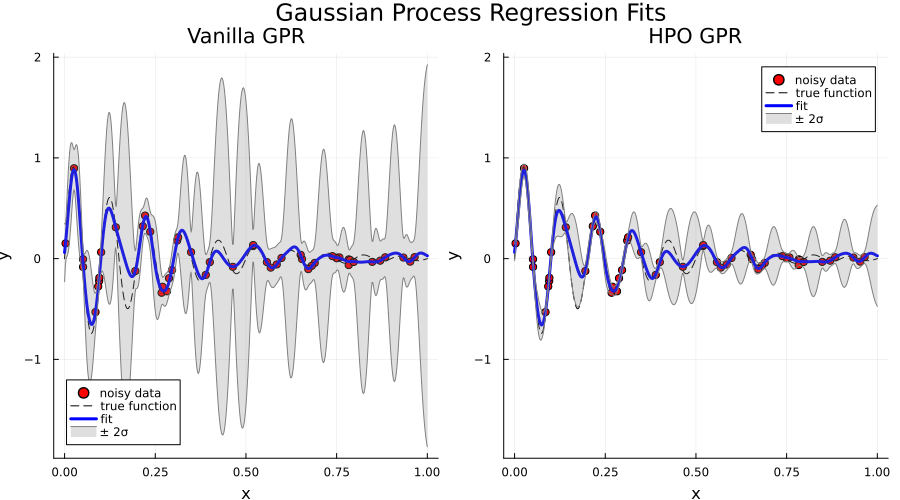
\includegraphics[width=0.85\columnwidth]{ml-figures/gpr/hpo-fit}
  \caption{Left: the original Gaussian Process obtained with our default choice of kernel parameters. Right: A much better Gaussian Process obtained after performing hyper-parameter optimization on the kernel parameters. Note how the mean function still does an excellent job fitting the data points while \textit{also} minimizing the uncertainty of the fit.}
  \label{fig:gpr-fit-comparison}
\end{figure}

To enable easy application of Gaussian Process Regression in Julia's machine learning framework \texttt{MLJ.jl}, we have created an open-source implementation which is made freely available at \url{https://github.com/john-waczak/MLJGaussianProcesses.jl/tree/main}

\subsection{Decision Trees}


%------------------------------------------------------------------------------------------%

\section{Unsupervised Classification}

%% \subsection{k-Means Clustering}

\subsection{Self Organizing Maps}

Self organizing maps (SOMs) are an unsupervised machine learning technique developed by Kohonen \cite{kohonen-original} based on the simple biological principle that \textit{neurons near each other fire together}. This observation that the toplogical \textit{closeness} of similar computational units is a critical feature of intelligent systems leads to a natural reinterpretation of the familiar perceptron model into a new form amenable for a variety of clustering and dimensionality reduction tasks. In particular, the SOM enables a rapid unsupervised classification of multidimensional data into a (typically) one or two dimensional \textit{simplicial complex}, the discrete realization of a topological manifold, whose vertices correspond to representative points in the original data space $\mathcal{D}$. While a tad esoteric compared to other popular unsupervised methods like KMeans clustering or DBSCAN, the SOM distinguishes itself with the added benefit that it's training procedure guarantees nodes (i.e. classes) close to each other in the feature manifold share similar weights. This additional structure makes the SOM particularly attractive when an interpretation of the discovered clusters as well as the relationships between them is desired.

The original treatment of the SOM by Kohonen was made in terms of processing units, sensory signals, and relaying networks \cite{kohonen-original}, however, in the modern era of deep learning, a more easily digestible derivation can be obtained by re-interpreting the weights of a simple perceptron model to provide the foundation for a clustering approach. As described in previously, a perceptron is a function of the form
\begin{equation}
    \mathbf{y} = \sigma.\left(W\mathbf{x}\right)
\end{equation}
where $W\in\mathbb{R}^{n\times m}$ is a matrix of weights which transform the input $\mathbf{x}\in\mathbb{R}^m$ into $\mathbb{R}^n$ and $\sigma$ is a nonlinear \textit{activation function} applied element-wise to the outputs of the matrix multiplication (indicated by the $.$ syntax). If we instead think of the weight matrix as an ordered collection of vectors $\{\mathbf{w}_i\}_{i=1}^{n}$, then this formula can be further decomposed into
\begin{equation}
    (\mathbf{y})_i = \sigma(\mathbf{w}_i^T\mathbf{x}) = \sigma(\langle \mathbf{w}_i, \mathbf{x} \rangle)
\end{equation}
The function of the perceptron is now clear: given an input vector $\mathbf{x}$ and a collection of $n$-many weight vectors $\mathbf{w}_i$, compute the $n$-many inner products of $\mathbf{x}$ with each weight vector $\mathbf{w}_i$, apply the nonlinear activation function $\sigma$, and concatenate the results.

If we now allow ourselves to imagine the weight vectors $\mathbf{w}_i$ as members of the same vector space as the input $\mathbf{x}$, a reasonable question to ask is: \textit{how similar is the input $\mathbf{x}$ to each $\mathbf{w}_i$}. Further, the application of the inner product $\langle \cdot,\cdot \rangle$ suggests we may answer this question in terms of the distance
\begin{equation}
    \langle \mathbf{w}_i-\mathbf{x},  \mathbf{w}_i-\mathbf{x}\rangle = d(\mathbf{w}_i, \mathbf{x})^2.
\end{equation}
In other words, given a set of weight vectors $\mathbf{w}_i$ which we may now think of as the cluster centers for our unsupervised model, we can measure the similarity between a given datum $\mathbf{x}_j$ and each cluster by computing the distance
\begin{equation}
    d_{ij} = d\left(\mathbf{w}_i, \mathbf{x}_j \right).
\end{equation}

To make this mapping useful, we should prescribe a \textit{training procedure} which updates the vectors $\mathbf{w}_i$ based on all of the available data points. Further, our goal is to establish some kind of interpretable relationship between the various weights $\mathbf{w}_i$ so that they \textit{more than} disjoint classes. The SOM achieves this by providing a lower-dimensional grid (typically 2-dimensional) whose vertices are understood to be the location of each of the weight vectors. The procedure is as follows:

First, initialize a grid of weight vectors $\mathbf{w}_i\in\R^m$ which we collect into a matrix $W\in\R^{m\times n}$. Assign coordinates to each weight vector by mapping each $\mathbf{w}_i$ to a vertex in the grid. The \textit{topology} of the grid is a hyperparameter which dictates the spatial relationship between neighboring nodes. Popular choices are: flat rectangular, rectangular on a cylinder (one periodic boundary condition), rectangular on a torus (two periodic boundary conditions), hexagonal (more equidistant neighbors per node than rectangular), and spherical.
\begin{figure}[h]
  \centering
  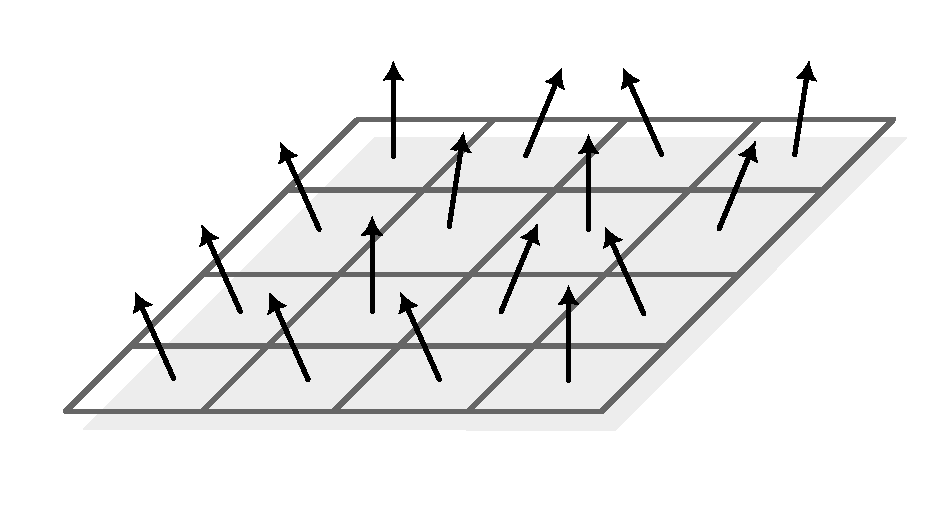
\includegraphics[width=0.75\columnwidth]{ml-figures/som/som-diagram.pdf}
  \caption{A Self Organizing Map with nodes configured in a rectangular grid topology with weight vectors randomly initialized.}
  \label{fig:som-diagram}
\end{figure}
One can initialize the weights in a variety of ways. Some common choices are
\begin{itemize}
\item Randomly initialize them as in figure \ref{fig:som-diagram}.
\item Initialize them to the value of $n$-many randomly selected data samples $\mathbf{x}_i$.
\item Initilize them to the first $n$-many principal components of the dataset.
\end{itemize}

Next, we proceed to update the weights according to the following steps for each $\mathbf{x}_k$ datum:
\begin{enumerate}
\item Compute the \textit{best match unit} (BMU) as
  \begin{equation}
    \mathbf{w}_{i}^{\text{best}} = \text{arg}\min\limits_{\mathbf{w}_j} \left( d(\mathbf{x}_k, \mathbf{w}_j)^2 \right)
  \end{equation}
  where $d(\cdot,\cdot)$ is some suitably chosen distance function. One often defaults to the Euclidean metric.
\item Choose a radius $\sigma_t$ which we will use to identify the correct update for to apply to all nodes relative to $\mathbf{w}_i^{\text{best}}$.
\item Update \textit{all} the weights according to the equation
  \begin{equation}
    w_{m}^{t+1} = w_m^{t} + \eta(t)f(x_m,y_n,\sigma_t)\left(\mathbf{x}_k  - \mathbf{w}_n^{t} \right)
  \end{equation}
  where $\eta(t)$ is the learning rate, and $f(x_m, y_m, \sigma_t)$ is the \textit{neighborhood} function which defines the relative amount each node $\mathbf{w}_m$ is updated according to its coordinate distance from the best match unit (i.e. the distance between the points $(x_m, y_m)$ and $(x_{\text{best}}, y_{\text{best}})$ in the two dimensional case). Typically one chooses a the learning rate to evolve according to the schedule
  \begin{equation}
    \eta(t) = \eta_0\exp(^-\lambda t)
  \end{equation}
  with the radius $\sigma_t$ evolving similarly according to
  \begin{equation}
    \sigma_t = \sigma_0\exp(-\beta t).
  \end{equation}
  Popular choices for the neighborhood function are the Gaussian function, Mexican-hat function, a cone function, and a cylinder function.
\end{enumerate}

\subsubsection{A simple example: partitioning color spaces}

As an illustrative example, consider the minimal dataset formed by the colors red, green, and blue which as vectors may be written as
\begin{align}
  \text{Red} &= \left(1,\; 0,\; 0 \right)\\
  \text{Green} &= \left(0,\; 1,\; 0 \right) \\
  \text{Blue} &= \left(0,\; 0,\; 1 \right).
\end{align}
Now let us suppose we want to train an SOM to generate a classification for colors using only these three as the supplied training data. Figure \ref{fig:som-demo} shows exactly this. Here we have trained an SOM of size $25 \times 25$ cells in a flat hexagonal topology. As the weight vectors are themselves vectors of length $3$, we can then visualize the trained SOM by coloring each corresponding node by the color learned in its weight vector. What we find is that the resulting map has clearly separated red, green, and blue into distinct regions in the grid, and more importantly, there is a smooth gradient between neighboring cells reflecting the fact that neighboring classes are more \textit{similar} than cells with a large separation distance. This is not the case for many other common clustering techniques like k-nearest neighbors or DBSCAN for which relationship between learned classes is challenging to interpret.

\begin{figure}[h!]
  \centering
  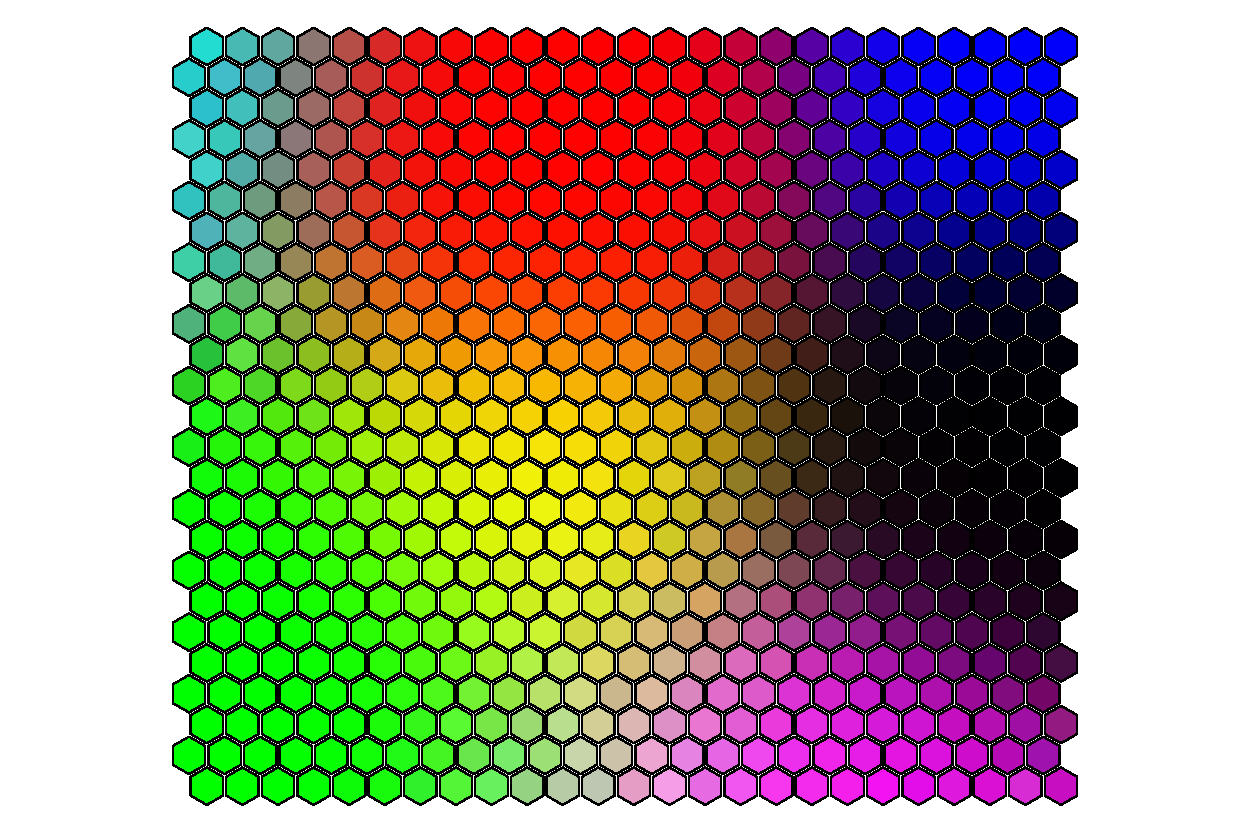
\includegraphics[width=0.75\columnwidth]{ml-figures/som/SOM_demo.pdf}
  \caption{A trained Self Organizing Map of $25\times 25$ cells in a hexagonal topology trained on a dataset consisting of the three colors red, green, and blue.}
  \label{fig:som-demo}
\end{figure}

To enable this demonstration and its subsequent use throughout the rest of this dissertation, I have created a new open-source implementation of the SOM algorithm for the Julia programming language called \texttt{SelfOrganizingMaps.jl} which has been added to the general registry and can by freely downloaded for use by anyone. The repository for the code as well as the associated documentation can be found at \href{https://github.com/john-waczak/SelfOrganizingMaps.jl}{this site}.

\subsection{Generative Topographic Maps}

Now that we've developed the SOM algorithm, we see upon reflection that there are a few drawbacks to the methods, namely
\begin{itemize}
\item There is no probabilistic interpretation of the fitted SOM? Are we to trust the fit results with $100\%$ certainty?
\item There is no clearly stopping criteria for the learning process? How many epochs should be performed? Do you simply stop the training once the neighbor radius $\sigma_t$ is less than the minimum neighbor distance?
\end{itemize}
With this in mind, we now seek to introduce a new method based on the SOM which will allow us to address the shortcomings by taking a principled, probabilistic approach, which will be called the \textit{Generative Topographic Mapping} (GTM). This technique was first introduced by Bishop et al. in  \cite{gtm-orig} and our derivation of the method will follow their presentation closely.

Both the SOM and GTM rely on the assumption that our high dimensional dataset $\D\subseteq\R^D$ can be accurately represented as being constrained to a lower dimensional submanifold. In the SOM this is acheived by assigning coordinates to each of the weight vectors according to some predetermined grid. In the GTM, however, we make a slight change in our perspective and say that the high dimensional data we have are \textit{generated} from some lower dimensional set of \textit{latent vectors} living in $\R^L$ with $L < D$. For ease of visualization, it is standard to chose $L=2$. Our goal, then, is to learn a mapping from the latent space to the data space which \textit{maximizes the likelihood} of obtaining our dataset given the set of latent variables.

In the coming derivation, we shall assume the following notations:
\begin{equation}
  \begin{aligned}
    \mathbf{x}\in\R^L &\quad \text{A latent vector} \\
    \mathbf{t}\in\R^D &\quad \text{A data vector}\\
    \mathbf{y}=\mathbf{y}(\mathbf{x};W) &\quad \text{The transformation } \mathbf{y}:\R^L\to\R^D \\
    W &\quad \text{The model weights}
  \end{aligned}
\end{equation}

To get started, let us assume that our data can be reasonably described by a multivariate normal distrubtion such that
\begin{equation}
  p(\mathbf{t} \vert \mathbf{x}; W, \beta) = \N\left(\mathbf{y}(\mathbf{x};W), \frac{1}{\beta}\right),
\end{equation}
that is, our data follow a normal distribution with mean given by the transformation function $\mathbf{y}$ applied to the latent variables $\mathbf{x}$ with covariance $\mathbf{1}{\beta}$. Suppose that we have some model for the prior distribution of our latent variables, $p(\mathbf{x})$, then by integration would find
\begin{equation}
  p(\mathbf{t}\vert W, \beta) = \int d\mathbf{x} p(\mathbf{t}\vert \mathbf{x};W,\beta) p(\mathbf{x})
\end{equation}
which is the distribution we really care about, namely, the distribution of data $\mathbf{t}\in\D$ given our choice of model weights $W$ and covariance $\beta^{-1}$. To make the problem tractible, we need an integrable distribution for $p(\mathbf{x})$. We therefore take inspiration from the SOM and choose $\mathbf{x}$ to be precisely distributed over a regular grid of points with equal weights. That is
\begin{equation}
  p(\mathbf{x}) = \frac{1}{K}\sum_k^K\delta(\mathbf{x}-\mathbf{x}_k)
\end{equation}
where $\mathbf{x}_k$ are the $K$-many grid points such that for any $\mathbf{x}$, there is a probability of precisely $\mathbf{1}{K}$ that it \textit{came from} one of the nodes $\mathbf{x}_k$.

\textcolor{red}{NOTE: Add figure of GTM grid here. (See pg 27 of notebook)}

As mathematicians (or physicists, or data scientists, etc...) we rejoice at the wise decision to incorporate the integral-zapping Dirac-delta distributions which enables us to simplify the data distribution to become
\begin{equation}
  \begin{aligned}
    p(\mathbf{t}\vert W, \beta) &= \int d\mathbf{x} p(\mathbf{t}\vert\mathbf{x};W,\beta)\frac{1}{K}\sum_k^K\delta(\mathbf{x}-\mathbf{x}_k) \\
    &= \frac{1}{K}\sum_k^Kp(\mathbf{t}\vert\mathbf{x}_k;W,\beta).
  \end{aligned}
\end{equation}

Now provided we have in supply a dataset with $N$-many records, i.e. $\D^N\subseteq\D =\{\mathbf{t}_1,\mathbf{t}_2,...,\mathbf{t}_N \}$, how do we chose the \textit{optimal} parameters $W$ and $\beta$? We need an objective to optimize!

If we assume the $\mathbf{t}_i$ are independently, identically distributed, then the \textit{likelihood} of obtaining the data given a choice of parameters (i.e. $p(\D^N\vert W,\beta)$) is
\begin{equation}
  \begin{aligned}
  \mathcal{L}(W,\beta) &= \prod\limits_{n}^N p(\mathbf{t}_n \vert W,\beta) \\
  &= \prod\limits_n^N \left(\frac{1}{K}\sum_k^K p(\mathbf{t}_n \vert \mathbf{x}_k; W, \beta) \right).
  \end{aligned}
\end{equation}

Taking the logarithm (which must share the same optimum as it is a monotonically increasing function) yields the simpler expression
\begin{equation}
  \ell(W,\beta) = \log(\mathcal{L}(W,\beta)) = \sum_n^N\log\left(\frac{1}{K}\sum_k^K p(\mathbf{t}_n \vert \mathbf{x}_k; W, \beta \right)
\end{equation}
Maximizing this log-likelihood function is known as \textit{maximum likelihood estimation} (MLE). But how should we optimize this function? We could use techniques like gradient descent or ADAM, however the probabilistic nature of the GTM suggests we may be able to obtain an \textit{expectation-maximization} (EM) routine for a suitable choice of transformation $\mathbf{y}(\mathbf{x},W)$.

Suppose we already have some guesses $W_o$ and $\beta_o$ for the parameters ($o$ for \textit{old}). To simplify the derivation, we define $\theta_o=(W_o..., \beta_o)$. Then we can compute the responsibilities $r_{kn}$ as
\begin{equation}
  \begin{aligned}
    r_{kn} &:= p(\mathbf{x}_k \vert \mathbf{t}_n,\theta_o) \\
    &= \frac{p(\mathbf{t}_n\vert \mathbf{x}_k, \theta_o)p(\mathbf{x}_k \vert \theta_o)}{p(\mathbf{t}_n\vert\theta_o)} \\
    &= \frac{p(\mathbf{t}_n\vert \mathbf{x}_k,\theta_o)p(\mathbf{x}_k\vert \theta_o)}{\sum_{k'}^Kp(\mathbf{t}_n\vert \mathbf{x}_{k'},\theta_o)p(\mathbf{x}_{k'}\vert\theta_o)} \\
    &= \frac{p(\mathbf{t}_n\vert \mathbf{x}_k,\theta_o)\frac{p(\mathbf{x}_k,\theta_o)}{p(\theta_o)}}{\sum_{k'}^Kp(\mathbf{t}_n\vert \mathbf{x}_{k'},\theta_o)\frac{p(\mathbf{x}_{k'},\theta_o)}{p(\theta_o)}} \\
    &= \frac{p(\mathbf{t}_n\vert \mathbf{x}_k,\theta_o)p(\mathbf{x}_k,\theta_o)}{\sum_{k'}^Kp(\mathbf{t}_n\vert \mathbf{x}_{k'},\theta_o)p(\mathbf{x}_{k'},\theta_o)} \\
    &= \frac{p(\mathbf{t}_n\vert \mathbf{x}_k,\theta_o)p(\mathbf{x}_k)p(\theta_o)}{\sum_{k'}^Kp(\mathbf{t}_n\vert \mathbf{x}_{k'},\theta_o)p(\mathbf{x}_{k'})p(\theta_o)} \\
    &= \frac{p(\mathbf{t}_n\vert \mathbf{x}_k,\theta_o)p(\mathbf{x}_k)}{\sum_{k'}^Kp(\mathbf{t}_n\vert \mathbf{x}_{k'},\theta_o)p(\mathbf{x}_{k'})} \\
    &= \frac{p(\mathbf{t}_n\vert \mathbf{x}_k,\theta_o)\frac{1}{K}}{\sum_{k'}^K\mathbf{t}_n\vert \mathbf{x}_{k'},\theta_o)\frac{1}{K}} \\
    &= \frac{p(\mathbf{t}_n\vert \mathbf{x}_k,\theta_o)}{\sum_{k'}^K\mathbf{t}_n\vert \mathbf{x}_{k'},\theta_o)}
  \end{aligned}
\end{equation}
which we will soon utilize in our EM procedure.

Now, we must chose a form for the transformation $\mathbf{y}(\mathbf{x},W)$ after which we will have all of the information we need to perform the computation. A convenient choice is to use a kernelized regression strategy so that
\begin{equation}
  \mathbf{y} := \mathbf{\phi}^T(\mathbf{x})W
\end{equation}
where $W\in\R^{M\times D}$ are some constant parameters and $\mathbf{\phi}:\R^L\to\R^M$ is a transformation employing $M$-many basis functions $\phi_m$. To capture linear and nonlinear effects, we chose
\begin{equation}
  \phi_m(\mathbf{x}) = \begin{cases}
    \quad \exp(-\frac{\lvert \mathbf{x}-\mu_m\rvert^2}{2\sigma}), & m < M \\
    \quad 1, & m = M
  \end{cases}
\end{equation}
that is, $M-1$ Gaussians and a term for a bias offset. If we apply the transformation to each of the $K$-many latent nodes, then we may collect the resulting vectors into a matrix,
\begin{equation}
  Y = \Phi W,
\end{equation}
where $\Phi\in\R^{K\times M}$ with $\Phi_{km}=\phi_m(\mathbf{x}_k)$.

Now that we are able to compute the responsibilities of each latent node to the observed data (the expectation step), we need to compute the relevant derivatives which we will use in the maximization step. For this, we treat the responsibilities $r_{kn}$ as fixed, and solve for the relevant updates to $W$ and $\beta$ which make there derivatives $0$ and therefore optimize $\ell$. Let's begin by differentiating $\ell$ with respect to the weight matrix $W$. We have
\begin{align}
    0 &= \frac{\partial}{\partial W_{md}}\ell(W,\beta) \\
    &= \frac{\partial}{\partial W_{md}}\sum_n^N\log\left( \frac{1}{K}\sum_k^Kp(\mathbf{t}_n \vert \mathbf{x}_k; W, \beta \right) \\
    &= \sum_n^N \frac{1}{\frac{1}{K}\sum_{k'}^Kp(\mathbf{t}_n\vert \mathbf{x}_{k'};W,\beta)}\frac{1}{K}\frac{\partial}{\partial W_{md}}\sum_k^Kp(\mathbf{t}_n\vert \mathbf{x}_k;W,\beta)
\end{align}
Noting that $p(\mathbf{t}_n\vert\mathbf{x}_k;W,\beta)=\N(\mathbf{y}_k,\beta^{-1})$, then the derivative of the exponential yields
\begin{align}
  0 &= \sum_n^N\sum_k^K \frac{p(\mathbf{t}_n\vert\mathbf{x}_k;W,\beta)}{\sum_{k'}^Kp(\mathbf{t}_n\vert\mathbf{x}_{k'};W,\beta)}\frac{\partial}{\partial W_{md}}\left(-\frac{\beta}{2}\lvert \mathbf{t}_n-\mathbf{y}_k \rvert^2 \right) \\
  &= \sum_n^N\sum_k^K r_{kn}\frac{\partial}{\partial W_{md}}\left(-\frac{\beta}{2}\lvert \mathbf{t}_n-\mathbf{y}_k \rvert^2 \right) \\
  &= \sum_n^N\sum_k^K (-\beta) r_{kn} \sum_q^D(y_k^q-t_n^q)\frac{\partial}{\partial W_{md}}\sum_s^M \phi_s(\mathbf{x}_k)W_{sq} \\
  &= \sum_n^N\sum_k^K\sum_q^D(-\beta)r_{kn}(y_k^q-t_k^q)\sum_s^M \phi_s(\mathbf{x}_k)\delta_{sm}\delta_{qd} \\
  &= \sum_n^N\sum_k^K (-\beta)r_{kn}(y_k^d-t_k^d) \phi_m(\mathbf{x}_k) 
\end{align}

Looking closely at the above expression, we see that there are two free indices suggesting we may write the above as a matrix expression. To do so, let's introduce a diagonal matrix $G$ such that $G_{kk} = \sum_nr_{kn}$. Then upon rearrangement, we find
\begin{align}
  \sum_n^N\sum_k^K r_{kn}y_k^d\phi_m(\mathbf{x}_k) &= \sum_n^N\sum_k^K r_{kn}t_n^d\phi_m(\mathbf{x}_k) \\
  \sum_n\sum_k r_{kn}\left(\sum_sW_{sd}\phi_s(\mathbf{x}_k)\right)\phi_m(\mathbf{x}_k) &= \sum_n\sum_k r_{kn}t_n^d\phi_m(\mathbf{x}_k) \\
  \sum_n\sum_k\sum_s r_{kn}\Phi_{ks}W_{sd}\Phi_{km} &= \sum_n\sum_k r_{kn}t_n^d\Phi_{km} \\
  \sum_k\sum_s \left( \sum_n r_{kn}\right)\Phi_{ks}W_{sd}\Phi_{km} &= \sum_n\sum_k r_{kn}t_n^d\Phi_{km} \\
  \sum_k\sum_s G_{kk}\Phi_{ks}W_{sd}\Phi_{km} &= \sum_n\sum_k r_{kn}t_n^d\Phi_{km} \\
  \sum_k\sum_s (\Phi_{km})^TG_{kk}\Phi_{ks}W_{sd} &= \sum_n\sum_k (\Phi_{km})^Tr_{kn}t_n^d \\
  \left( \Phi^TG\Phi W \right)_{md} &= \left( \Phi^TRT \right)_{md}
\end{align}
where we have defined $T_{nd}=t_n^d$ and $R_{kn} = r_{kn}$.

By the same procedure, we find that differentiation with respect to $\beta$ leads to
\begin{equation}
  \frac{1}{\beta} = \frac{1}{ND}\sum_n^N\sum_k^K r_{kn}\lvert \mathbf{y}_k-\mathbf{t}_n\rvert^2
\end{equation}
so that together the maximization step amounts to solving
\begin{equation}
  \begin{cases}
    \quad \Phi^TG_{\text{old}}\Phi W_{\text{new}} = \Phi^T R_{\text{old}} T \\
    \quad \dfrac{1}{\beta_{\text{new}}} = \dfrac{1}{ND}\sum\limits_n^N\sum\limits_k^KR_{kn}^{\text{(old)}}\lvert \mathbf{y}_k - \mathbf{t}_n \rvert^2
  \end{cases}
\end{equation}

The last piece we need for the training algorithm is a method to initialize the parameters $W$ and $\beta$. As before with the SOM, there are a few different options. In particular we might
\begin{itemize}
  \item Randomly initialize the weight matrix $W$
  \item Use PCA to initialize the weights to a linear model. To do this, one computes the data covariance matrix $U$ keeping only the first two columns. We then initialize $W$ so that
      \begin{equation}
        W\Phi^T \approx UX^T
      \end{equation}
      and then set $\beta^{-1}$ to the third principal component variance.
\end{itemize}

In summary, the GTM training procedure is as follows
\begin{enumerate}
  \item Generate a grid of latent points $\{\mathbf{x}_k\}_{k=1}^K$.
  \item Generate basis function centers $\{\mu_m\}_{m=1}^M$.
  \item Select an basis function width $\sigma$.
  \item Compute the matrix of activations $\Phi$ where
    \begin{equation}
      \Phi_{mk} = \Phi_m(\mathbf{x}_k)
    \end{equation}
  \item Initialize the weight matrix $W$ randomly or with PCA
  \item Initialize $\beta$ randomly or with PCA
  \item (Optional) select a value for $\alpha$ to enable weight regularization, i.e. $(\Phi^TG\Phi + \frac{\alpha}{\beta}I)W=\Phi^TRT$. This corresponds to specifying a prior distribution on the weights $W$ such that $p(W)\propto \exp(-\alpha||W||^2/2)$.
  \item Compute the difference matrix $\Delta := \lvert T - \Phi W\rvert^2$
  \item Repeat the following until convergence:
    \begin{enumerate}
      \item (Expectation step) Compute the responsibility matrix $R$ using $\Delta$ and $\beta$.
      \item Compute $G$ from $R$
      \item (Maximization step) Compute the update to the weight matrix $W$ with $W_{\text{new}} = \left(\Phi^TG\Phi\right)^{-1}\Phi^TRT$
      \item Compute the updated difference matrix $\Delta$
      \item Compute the updated $\beta$
    \end{enumerate}
\end{enumerate}

Excellent! We now have a robust procedure to fit the GTM model. With a fitted GTM in hand, how do we utilize the results? The main idea is that the fitted GTM provides us all of the relevant probability distributions to explain how we obtained our current data $\mathbf{t}_n$ from the latent vectors $\mathbf{x}_k$. Using Baye's rule, we can invert this relationship using our responsibility matrix $R$ to understand the contributions of each latent vector $\mathbf{x}_k$ to each data. Since this would lead to a different $R$ matrix for each datapoint, one often computes a handful of summary statistics using $R$ rather then using the entire result. For example, we find the mean of the distribution to be
\begin{equation}
  \begin{aligned}
    \langle \mathbf{x} \vert \mathbf{t}_n; W,\beta\rangle &= \int d\mathbf{x} p(\mathbf{x}\vert\mathbf{t}_n;W,\beta)\mathbf{x} \\
    &= \int d\mathbf{x}\frac{p(\mathbf{t}_n\vert\mathbf{x};W,\beta)p(\mathbf{x})}{\int d\xi p(\mathbf{t}_n\vert \xi; W,\beta)p(\xi)}\mathbf{x} \\
    &= \int \sum_k \frac{p(\mathbf{t}_n\vert \mathbf{x},W,\beta)\mathbf{x}\delta(\mathbf{x}-\mathbf{x}_k)}{\sum_{k'}p(\mathbf{t}_n\vert\mathbf{x}_{k'};W,\beta)} d\mathbf{x}  \\
    &= \sum_k \frac{p(\mathbf{t}_n\vert \mathbf{x}_k; W, \beta)\mathbf{x}_k}{\sum_{k'}p(\mathbf{t}_n\vert\mathbf{x}_{k'};W,\beta)} \\
    &= \sum_k^K R_{kn}\mathbf{x}_k
  \end{aligned}
\end{equation}
However, in cases where the distribution is multi-modal, the mean can be misleading. It can therefore also be useful to compute the mode of the distribution which is given by
\begin{equation}
  \mathbf{x}_{\text{mode}} = \mathbf{x}_{k_\text{max}}
\end{equation}
where $k_{\text{max}} = \text{arg}\max_{k}(R_{kn})$.

To provide an easy to use open-source implementation of the GTM algorithm, I have created a publicly accessible github repo with a Julia implementation that comports with the \texttt{MLJ.jl} machine learning framework. The repo can be found \href{https://github.com/john-waczak/GenerativeTopographicMapping.jl/tree/main}{here} and makes it easy to incorporate GTMs into complicated machine learning pipelines.

\textcolor{red}{UPDATE REQUIRED: Add demo use for GTM like we did for the SOM}.

%------------------------------------------------------------------------------------------%

%% \section{Dimensionality Redution}
%% \subsection{PCA}
%% \subsection{ICA}
%% \subsection{t-SNE}


%------------------------------------------------------------------------------------------%

%% \section{Model Ensembling}
%% MLJ and SciKitLearn documentation sites will have good references for this, I think.
%% \subsection{Bagging}
%% e.g. Random Forests
%% \subsection{Boosting}
%% e.g. XGBoost
%% \subsection{Stacking}
%% e.g. Super Learners. Use the example of model stacking from MLJ documentation to describe our approach.



%------------------------------------------------------------------------------------------%

\section{Uncertainty Quantification via Conformal Prediction}

Having established a variety of machine learning methods which we will use throughout the rest of this dissertation, a natural next question is: How can we evaluate our confidence in the predictions of machine learning models? For some methods like Gaussian Process Regression, our models naturally output distributions which we can evaluate to provide predictions via the mean, and uncertainty estimates via the standard deviation or some similar statistic. For models like Neural Networks and Decision Tress which are not inherently probabilistic, there is no obvious way to extract uncertainty estimates purely from the model's predictions. One standard approach is to attempt to evaluate our confidence in a particular model by comparing the predictions of many copies of the same model trained on complementary cross validation folds of the original training set. By examining the prediction variance due to variation in the supplied training data, we can establish some expectation for uncertainty in our model's output.

Clearly this approach is far from perfect. Therefore, in order to prevent ourselves from biasing towards using only those methods like Gaussian Process Regression which output distributions by default, we would like to develop a robust procedure for augmenting \textit{any} regression model with the capability to simultaneously estimate target values and\textit{confidence intervals} by taking advantage of our (often) large datasets to establish sufficient statistics. Further, we do not wish to make any assumptions about the particular target distributions; without sufficient reason to expect a variable to be normally distributed why should we make this \textit{strong} assumption? This is the approach taken by \textit{Conformal Prediction} which we will develop in this section and utilize throughout the rest of this dissertation. 

\begin{figure}[h]
  \centering
  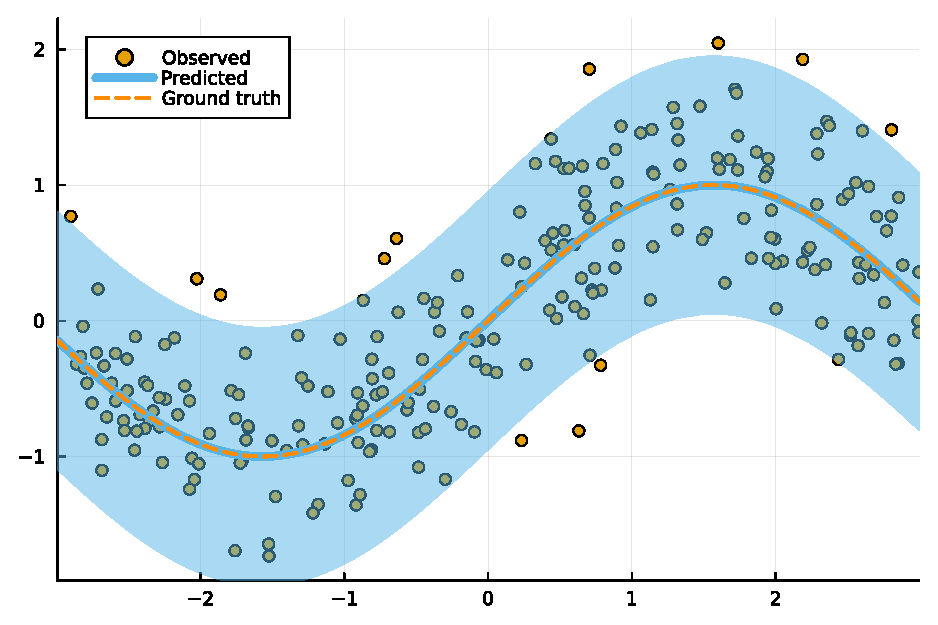
\includegraphics[width=0.75\columnwidth]{ml-figures/conformal-prediction/cp-demo.pdf}
  \caption{An example of conformal prediction for a model estimating a noisy one-dimensional target. The blue shaded region illustrates the learned confidence interval. Image taken from  \cite{conformalprediction.jl}}
\end{figure}


As discussed in the previous section, the typical machine learning procedure involves partitioning our dataset into independent training and testing batches (or $k$-many cross-validation folds) so that we can evaluate a trained model's performance and ensure we have not run afoul of over/under-fitting. In conformal prediction, we introduce an additional split so that our original dataset $\D$ can be decomposed into $\D = \D_{\text{train}}\cup \D_{\text{cal}} \cup \D_{\text{test}}$. We then start with \textit{any} heuristic notion of model uncertainty, and make the estimated confidence interval rigorous by adjusting the output to \textit{guarantee} the desired coverage is satisfied on the calibration set $\D_{\text{cal}}$.

A high level outline of the procedure is as follows
\begin{enumerate}
\item Define a score function $s(x,y)\in\R$ using some heuristic notion of uncertainty so that large $s$ means \textit{worse} agreement between $\hat{f}(x)$ and the target $y$.
\item Compute $\hat{q}$ as the $\dfrac{\lceil (n+1)(1-\alpha) \rceil}{n}$ quantile of the scores $s_i = s(x_i, y_i)$ generated from the calibration set $\D_{\text{cal}}$.
  \item Use $\hat{q}$ to form valid prediction intervals.
\end{enumerate}

The question then becomes: How can we obtain accurate uncertainty estimates if the score function $s$ need not be accurate? So long as the scores $s_i$ accurately rank estimates from best to worst model error, then all we need to do is \textit{calibrate} the scores to achieve a confidence interval with the desired coverage, i.e. so that the interval is always large enough to guarantee the coverage we require. It may be that our predicted interval is \textit{too large} for a poor scoring function. As an example, let's demonstrate how we can form correct estimates for the specific problem of quantile regression.

\subsection{Conformalizing Quantile Regression}

In quantile regression the goal is to predict the $\gamma^{th}$ quantile of the targets $y$ given the input features $x$. Let us denote $t_\gamma(x)$ as the true value for the $\gamma^{th}$ quantile and $\hat{t}_\gamma(x)$ as our predicted value. In this framework, we could then expect the interval $[t_{0.05}, t_{0.95}]$ to constitute a $90\%$ coverage confidence interval. However, our fitted values $\hat{t}_\gamma$ will certainly be imperfect so that the actual interval obtained will not conform to the desired $90\%$. Suppose we have a holdout dataset $\D_{\text{cal}}$ as previously mentioned, and for notational consistency, let $\alpha$ be the coverage so that we may write our predicted interval as $[\hat{t}_{\alpha/2}, \hat{t}_{1-\alpha/2}]$. A reasonable score function (i.e. uncertainty heuristic) would be
\begin{equation}
  s(x,y) = \max\left\{\hat{t}_{\alpha/2}(x)-y, y-\hat{t}_{1-\alpha/2}(x) \right\}
\end{equation}
so that the score is the distance to the nearest of our predicted quantiles. From this score, we may then form
\begin{equation}
  \hat{q} = \text{Quantile}\left(\left\{ s(x_i,y_i) \vert (x_i,y_i)\in\D_{\text{cal}}\right\}, \frac{\lceil (n+1)(1-\alpha) \rceil}{n}\right),
\end{equation}
that is, $\hat{q}$ is the  $\frac{\lceil (n+1)(1-\alpha) \rceil}{n}$-th quantile of the scores from our calibration set. Using these corrections, we then output the \textit{conformalized} interval
\begin{equation}
  C(x) = \left[ \hat{t}_{\alpha/2}(x)-\hat{q}, \hat{t}_{1-\alpha/2}(x)+\hat{q} \right]
\end{equation}
which we have guaranteed achieves the desired coverage on the holdout set. If $\D_{\text{cal}}$ is sufficiently representative, then we will have achieved a rigorous interval for a coverage of $\alpha$. The effect is that $\hat{q}$ adjusts our previously estimated interval so that a positive $\hat{q}$ widens the interval and a negative $\hat{q}$ shrinks it in order to obtain the appropriate coverage.

How do we implement this in practice? Any model that we fit by minimizing the mean squared error (e.g. a Neural Network) can be agumented to instead fit the so-called \textit{pinball loss}
\begin{equation}
  L_\gamma(\hat{t}_{\gamma}, y) = \begin{cases}
    (y-\hat{t}_{\gamma})\gamma; & \hat{t}_{\gamma} < y \\
    (\hat{t}_{\gamma}-y)(1-\gamma); & \hat{t}_{\gamma} \geq y
    \end{cases}
\end{equation}
For $\gamma=0.5$, this reduces to the standard $\ell_1$ loss $\ell_1(\hat{t},y) = \lvert \hat{t}-y\rvert/2$ which encourages models to learn the median (i.e. the $0.5$ quantile).

\textcolor{red}{NOTE: Add plot of pinball loss for reference}

\subsection{Conformalizing Scalar Uncertainty Estimates}

Another common method for producing uncertainty estimates it to simultaneously predict the mean and standard deviation of the target distribution by assuming a Gaussian shape. More generally, we may seek to estimate a model uncertainty directly by first training a model, $\hat{f}(x)$, to predict the target $y$, and then train a second model $\hat{r}(x)$ to predict the residual error, that is
\begin{equation}
  \hat{r} = \lvert y - \hat{f}(x)\rvert.
\end{equation}
In either case, one could then form a confidence interval as
\begin{equation}
  \left[ \hat{f}(x) - \hat{r}(x), \hat{f}(x) + \hat{r}(x) \right].
\end{equation}

Other reasonable approaches to extract a heuristic uncertainty from a trained model might include
\begin{itemize}
\item Compute the output variance of an ensemble model $\hat{f}$
\item Compute the prediction variance obtained when randomly dropping out nodes from a neural network.
\item Estimate the variance of $\hat{f}$ resulting from small perturbations of the input $x$.
\end{itemize}
For all of these cases, we may call the uncertainty estimate $u(x)$ and form the score function
\begin{equation}
  s(x,y) = \frac{\lvert y - \hat{f}(x) \rvert}{u(x)}
\end{equation}
so that the score function $s$ measures how well our uncertainty estimate $u(x)$ matches the actual error $\lvert y -\hat{f}(x)$. If the error is large our predicted uncertainty is small, then $s$ will be large. Consequently, the score function tells us the correction we must apply to our estimate $u(x)$ in order to predict the actual model error, that is,
\begin{equation}
  \lvert y - \hat{f}(x) \rvert = s(x,y)u(x).
\end{equation}

If we now take $\hat{q}$ to be the $\frac{\lceil(n+1)(1-\alpha) \rceil}{n}$-th quantile as before, we are guaranteed that
\begin{equation}
  p(s(x_{\text{cal}}, y_{\text{call}}) \leq \hat{q}) \geq 1 - \alpha
\end{equation}

An easy-to-use implementation of these methods is provided by the open-source Julia package \texttt{ConformalPrediction.jl} which is designed to integrate into the larger \texttt{MLJ.jl} machine learning framework. We will utilize these techniques throughout the remainder of this dissertation in order to establish uncertainty estimates for \textit{all} of our regression models.


%% \textcolor{red}{UPDATE REQUIRED: we should add a couple more paragraphs referencing the key papers that develop this technique as well as a few example use cases it has been applied to}.

%------------------------------------------------------------------------------------------%

%% \section{Scientific Machine Learning}
%% \subsection{Physics-Informed Neural Networks}
%% \subsection{Universal Differential Equations}

%% \subsection{Hamiltonian Neural Networks}
%% We can save this section for the time-series results


%------------------------------------------------------------------------------------------%

%% \section{Generative Methods}
%% \subsection{Auto Encoders}
%% \subsection{Generative Adversarial Networks}


%------------------------------------------------------------------------------------------%

\section{Data Assimilation}

%% \textcolor{red}{NOTE: We should add further derivations from a Bayesian framework to fit in with what we've done for the Gaussian process regression and generative topographic maps. We should also add some more generic background to the topic of Data Assimilation, it's first uses in Meteorology, }


The proper application of scientific models to make real-world predictions requires that we commit ourselves to a full accounting of all possible sources of uncertainty when reporting results. Further, the explosion of \textit{big data} across scientific fields provieds a plethora observational data that our models are typically unequipped to incorporate when making predictions. The field of \textit{Data Assimilation} addresses this problem by providing a family of techniques engineered to combine model output together with observational data whilst enabling a complete accounting the sources of uncertainty. For chaotic systems in particular, data assimilation enables integration on long time scales that would be impossible via models alone. In this overview, we will follow the examples from \cite{pyda}.

Data assimilation can be cleanly developed in the framework of discrete dynamical systems. Since, at the end of the day, all of our scientific models must be discretized to be evaluated numerically, this is a reasonable course of action. Our goal is to find the best prediction for the system state vector $u$ that combines our model predictions, also known as \textit{forecasts}, with observational data. Model predictions are described via the discrete update equation:
\begin{equation}
    u_{k+1} = \mathcal{M}(u_k; \theta)
\end{equation}
For ODE systems, $\mathcal{M}$ represents the time integration scheme for a models like
\begin{equation}
    \dfrac{du}{dt} = f(u, t; \theta),
\end{equation}
in other words, a particular choice of ODE integration scheme (Runge Kutta for example) used to evolve the state vector $\u$ from time $u_k$ to $u_{k+1}$.

To measure the performance of our assimilation scheme, we denote the \textit{true} value of the state vector as $u^{(t)}$. The output of our model is denoted $u^{(b)}$ (\textit{b} superscript for \textit{background}). The discrepancy between the true value and our forecast is denoted $\xi^{(b)} = u^{(t)} - u^{(b)}$ characterizing the extent to which our model prediction is imperfect. The observations of our system are denoted by $w_k = w(t_k)$. These observations do not necessarily need to be components of the state vector $u$, but rather, are related to it via the \textit{observation function}, $h:u_k\mapsto w_k$. For example, one may attempt to predict surface sea temperatures using data assimilation with data from satellite observations. The function $h$ would then be the Stefan-Boltzmann relating the measured spectra to temperature. However, real world data is \textit{also} imperfect, which we must take into account let we over constrain our model with poor quality data. We write
\begin{equation}
    w_k = h(u_k) + \xi_k^{(m)}
\end{equation}
where $\xi_k^{(m)}$ denotes this measurement error.

Given our model predictions $u_{k}^{(b)}$ and observations $w_k$, we seek to obtain the \textit{optimal} or best-possible prediction called the \textbf{analysis}, $u^{(a)}$. Despite our care, this analysis will still be imperfect, so we further define the analysis error as
\begin{equation}
\xi^{(a)} = u^{(t)} - u^{(a)}
\end{equation}

In summary, we have defined the following relevant quantities (at time $t_k$):
\begin{align}
  &u_k^{(t)} \in \mathbb{R}^n &\text{the true state vector} \\
  &u_k^{(b)} \in \mathbb{R}^n &\text{the model forecast} \\
  &u_k^{(a)} \in \mathbb{R}^n &\text{the analysis} \\
  &w_k \in \mathbb{R}^m &\text{the observation vector} \\
  &\xi^{(b)} \in \mathbb{R}^n &\text{the model forecast error}\\
  &\xi^{(m)} \in \mathbb{R}^m &\text{the observation noise vector}\\
  &\xi^{(a)} \in \mathbb{R}^n &\text{the analysis error}\\
  &\xi^{(p)} \in \mathbb{R}^n &\text{the process noise if we used our model on the true state}\\
  &\mathcal{M}:\mathbb{R}^n\to\mathbb{R}^n &\text{the discrete model evolution function}\\
  &f:\mathbb{R}^n\to\mathbb{R}^n &\text{differential equation model (the right hand side)}\\
  &h:\mathbb{R}^n\to\mathbb{R}^m  &\text{observation function}
\end{align}

To move forward, we now establish the following (prior) assumptions about the distribution of errors in each component in order to make it possible to derive a closed form for the final analysis. We require
\begin{align}
  &\E[\xi_k^{(b)}] = 0 & &\E[\xi_k^{(b)}(\xi_j^{(b)})^T] = 0 \text{ for } k\neq j\\
  &\E[\xi_k^{(m)}] = 0 & &\E[\xi_k^{(m)}(\xi_j^{(m)})^T] = 0 \text{ for } k\neq j\\
  &\E[\xi_k^{(b)}(u_0)^T] = 0 & &\E[\xi_k^{(m)}(u_0)^T] = 0\\
  &\E[\xi_k^{(b)}\xi_j^{(m)}] = 0 & &  % \\
  %% &\E[u_k^{(t)}] = u_k^{(b)} & &
\end{align}
or in words, the errors in our model and observation are unbiased (e.g. mean zero) and uncorrelated.

We also define the error covariance matrices
\begin{align}
  Q_k &:= \E[\xi_k^{(p)}(\xi_k^{(p)})^T] \\
  R_k &:= \E[\xi_k^{(m)}(\xi_k^{(m)})^T] \\
  B_k &:= \E[\xi_k^{(b)}(\xi_k^{(b)})^T]
\end{align}
which we will use in our consideration of the final error of our analysis.

\subsection{Kalman Filter}
Given some model for the error covariance matrices $Q_k$ and $R_k$, we would like a method that propagates \textit{both} our model \emph{and} the errors forward. This way we may guarantee that the accuracy of our analysis doesn't come at the cost of higher uncertainty.

The original implementation of the Kalman filter was for strictly linear systems, in particular as a filter for signal processing. We will first develop the analysis for this simplified case adn then will generalize to the \textit{Extended Kalman Filter} (EKF) that can handle fully nonlinear situations.

In the linear case, our system may be written as
\begin{align}
    u_{k+1}^{(t)} &= M_ku_k^{(t)} + \xi_{k+1}^{(p)} \\
    w_k &= H_ku_k^{(t)} + \xi_k^{(m)}
\end{align}
where $M_k$ and $H_k$ are now matrices defining the linear problem.

The goal of the Kalman filter is to derive the analysis $u^{(a)}$ which minimizes the trace of the analysis error covariance matrix (i.e. sum of squared errors): \begin{equation}
    \mathrm{Tr}\left( P_k\right) := \E[(u_k^{(t)}-u_k^{(a)})^T(u_k^{(t)}-u_k^{(a)})]
\end{equation}
Finding the analysis consists of two steps: the forecast step and the assimilation step.

Beginning with the forecasting step, assume we have the analysis at time $t_k$ denoted $u_k^{(a)}$. Then the forecast for time $t_{k+1}$ is
\begin{equation}
    u_{k+1}^{(b)} = M_ku_k^{(a)},
\end{equation}
or in words, we obtain the next prediction by evolving the previous analysis forward. The background error is therefore
\begin{align}
    \xi_{k+1}^{(b)} &= u_{k+1}^{(t)} - u_{k+1}^{(b)} \\
    &= M_ku_k^{(t)}+\xi_{k+1}^{(p)} - M_{k}u_k^{(a)} \\
    &= M_k\left(u_k^{(t)}-u_k^{(a)} \right) + \xi_{k+1}^{(p)} \\
    &= M_k\xi_k^{(a)} + \xi_{k+1}^{(p)}
\end{align}

We may now evaluate the covariance matrix of our background estimate as:
\begin{align}
    B_{k+1} &= \E[\xi_{k+1}^{(b)}(\xi_{k+1}^{(b)})^T] \\
    &= \E\left[\left(M_k\xi_k^{(a)} + \xi_{k+1}^p \right) \left(M_k\xi_k^{(a)} + \xi_{k+1}^p \right)^T \right] \\
\end{align}

If we presume that $\E[\xi_k^{(b)}(\xi_{k+1}^{(p)})^T] = 0$, then the cross terms vanish and we are left with
\begin{equation}
    \boxed{B_{k+1} = M_kP_kM_k^T + Q_{k+1}}
\end{equation}

Thus we now have the background (i.e forecast) estimate of the state at $t_{k+1}$ and its covariance matrix. Given a measurement $w_{k+1}$ at the same time with covariance matrix $R_{k+1}$, we may now perform the assimilation step where we fuse the two sources of information to obtain $u_{k+1}^{(a)}$ and $P_{k+1}$.

Let's suppose that the analysis has the form
\begin{equation}
    u_{k+1}^{(a)} = \nu + K_{k+1}w_{k+1}
\end{equation}

for some vector $\nu\in\R^n$ and matrix $K_{k+1}\in\R^{m\times n}$. In a perfect world, we would have $\E[u_{k}^{(t)}-u_{k}^{(a)}] = 0$. Therefore,

\begin{align}
    0 &= \E[u_k^{(t)} - u_k^{(a)}] \\
    &= \E[(u_k^{(b)} + \xi_k^{(b)}) - (\nu + K_kw_k)] \\
    &= \E[(u_k^{(b)} + \xi_k^{(b)}) - (\nu + K_kH_ku_k^{(t)} + K_k\xi_k^{(m)})] \\
    &= \E[u_k^{(b)}] + \E[\xi_k^{(b)}] - \E[\nu] -K_kH_k\E[u_k^{(t)}] - K_k\E[\xi_k^{(m)}]\\
    &= u_k^{(b)} + 0 - \nu - K_kH_ku_k^{(b)} - 0 \\
    &= u_k^{(b)} - \nu - K_kH_ku_k^{(b)} \\
    \Rightarrow \nu &= u_k^{(b)} - K_kH_ku_k^{(b)}
\end{align}

which we now substitute to obtain

\begin{equation}
    \boxed{u_k^{(a)} = u_k^{(b)} + K_k(w_k - H_ku_k^{(b)})}
\end{equation}

Now that we know the form for the analysis we may derive the optimal matrix $K_k$ by optimization of $P_k$. We have

\begin{align}
	\xi_k^{(a)} &= u_k^{(t)} - u_k^{(a)} \\
                &= M_{k-1}u_{k-1}^{(t)} + \xi_{k}^{(p)} - u_k^{(b)} - K_k\left(w_k - H_ku_k^{(b)} \right) \\
                &= M_{k-1}u_{k-1}^{(t)} + \xi_{k}^{(p)} - M_{k-1}u_{k-1}^{(a)} - K_k\left(H_ku_k^{(t)} + \xi_k^{(m)} - H_ku_k^{(b)} \right) \\
                &= M_{k-1}u_{k-1}^{(t)} + \xi_{k}^{(p)} - M_{k-1}u_{k-1}^{(a)} - K_kH_ku_k^{(t)} - K_k\xi_k^{(m)} + K_kH_ku_k^{(b)} \\
                &= M_{k-1}u_{k-1}^{(t)} + \xi_{k}^{(p)} - M_{k-1}u_{k-1}^{(a)} - K_kH_ku_k^{(t)} - K_k\xi_k^{(m)} + K_kH_ku_k^{(b)} \\
                &= \Big\{ M_{k-1}(\xi_{k-1}^{(a)}+u_{k-1}^{(a)}) + \xi_{k}^{(p)} - M_{k-1}u_{k-1}^{(a)} \Big\} - K_kH_ku_k^{(t)} - K_k\xi_k^{(m)} + K_kH_ku_k^{(b)} \\
                &= \Big\{ M_{k-1}\xi_{k-1}^{(a)} + \xi_{k}^{(p)} \Big\} - K_kH_ku_k^{(t)} + K_kH_ku_k^{(b)} - K_k\xi_k^{(m)}\\
                &= M_{k-1}\xi_{k-1}^{(a)} + \xi_{k}^{(p)} - K_kH_k(M_{k-1}u_{k-1}^{(t)} + \xi_k^{(b)}) + K_kH_ku_k^{(b)} - K_k\xi_k^{(m)}\\
                &= M_{k-1}\xi_{k-1}^{(a)} + \xi_{k}^{(p)} - K_kH_kM_{k-1}(\xi_{k-1}^{(a)} + u_{k-1}^a) - K_kH_k\xi_k^{(b)} + K_kH_ku_k^{(b)} - K_k\xi_k^{(m)}\\
                &= M_{k-1}\xi_{k-1}^{(a)} + \xi_{k}^{(p)} - K_kH_kM_{k-1}(\xi_{k-1}^{(a)} + u_{k-1}^a) - K_kH_k\xi_k^{(b)} + K_kH_kM_{k-1}u_{k-1}^{(a)} - K_k\xi_k^{(m)}\\
                &= M_{k-1}\xi_{k-1}^{(a)} + \xi_{k}^{(p)} - K_kH_kM_{k-1}\xi_{k-1}^{(a)} - K_kH_k\xi_k^{(b)} - K_k\xi_k^{(m)}\\
                &= \big(I-K_kH_k \big)(M_{k-1}\xi_{k-1}^{(a)} - \xi_{k}^p) - K_k\xi_k^{(m)}\\
\end{align}

and therefore the covariance matrix is

\begin{align}
    P_k &= \E[\xi_{k}^{(a)}(\xi_{k}^{(a)})^T] \\
        &= \E\Big[\left(\big(I-K_kH_k \big)(M_{k-1}\xi_{k-1}^{(a)} - \xi_{k}^p) - K_k\xi_k^{(m)} \right) \left(\big(I-K_kH_k \big)(M_{k-1}\xi_{k-1}^{(a)} - \xi_{k}^p) - K_k\xi_k^{(m)} \right)^T \Big] \\
        &= \big(I-K_kH_k \big)M_{k-1}\E[\xi_{k-1}^{(a)}(\xi_{k-1}^{(a)})^T]M_{k-1}^T\big(I-K_kH_k \big)^T \\
        &\qquad \qquad + \big(I-K_kH_k \big)\E[\xi_k^{(p)}(\xi_k^{(p)})^T]\big(I-K_kH_k \big)^T \notag\\
        & \qquad \qquad - K_k\E[\xi_{k}^{(m)}(\xi_k^{(m)})^T]K_k^T \notag\\
        &= \big(I-K_kH_k \big)B_k\big(I-K_kH_k \big)^T - K_kR_kK_k^T
\end{align}

Now all that remains is to derive the specific form for $K_k$. The Kalman filter is defined as that $K_k$ which which minimizes the sum of squared analysis errors, i.e. the trace of the analysis error covariance matrix. Therefore, the following identities from matrix calculus will be useful:
\begin{align}
    \mathop{\nabla}_{A}\text{tr}(AB) &= B^T \\
    \mathop{\nabla}_{A}\text{tr}(BA^T) &= B \\
    \mathop{\nabla}_{A}\text{tr}(ABA^T) &= AB^T + AB  \\
\end{align}
from which we obtain
\begin{align}
    0 &= \mathop{\nabla}_{K_k}\text{tr}(P_k) \\
      &= \mathop{\nabla}_{K_k}\Big\{ B_k -B_kH_k^TK_k^T - K_kH_kB_k  + K_kH_kB_kH_k^TB_k^T - K_kR_kK_k^T \Big\} \\
      &= -B_kH_k^T - (H_kB_k)^T + K_k\left[H_kB_kH_k^T + (H_kB_kH_k^T)^T - R_k+R_k^T\right] \\
      &= -2B_kH_k^T + 2K_k\left(H_kB_kH_k^2 - R_k \right) \\
  \Rightarrow K_k &= B_kH_k^T\Big[ H_kB_kH_k^T - R_k \Big]^{-1}
\end{align}
we now substitute this result to obtain a simplified form for $P_k$:
\begin{align}
    P_k &= \left(I - K_kH_k \right)B_k\left(I - K_kH_k \right)^T + K_kR_kK_k^T \\
        &= \left(I - K_kH_k \right)B_k - \left(I - K_kH_k \right)B_k\left(K_kH_k \right)^T + K_kR_kK_k^T \\
        &= \left(I - K_kH_k \right)B_k -\left\{ \left(I - K_kH_k \right)B_k\left(K_kH_k \right)^T + K_kR_kK_k^T \right\} \\
        &= \left(I - K_kH_k \right)B_k -\left\{ \left(I - K_kH_k \right)B_kH_k^TK_k^T + K_kR_kK_k^T \right\} \\
        &= \left(I - K_kH_k \right)B_k -\left\{ \left(I - K_kH_k \right)B_kH_k^T + K_kR_k \right\}K_k^T \\
        &= \left(I - K_kH_k \right)B_k -\left\{ B_kH_k^T - K_k\left( H_kB_kH_k^T + R_k \right)  \right\}K_k^T \\
        &= \left(I - K_kH_k \right)B_k -\left\{ B_kH_k^T - B_kH_k^T \right\}K_k^T \\
        &= \left(I - K_kH_k \right)B_k
\end{align}
where we have used the fact that covariance matrices are symmetric.


Now that we have all of the pieces, let's summarize the procedure:
\begin{enumerate}
\item \textbf{Initialization}: We must set the system to some initial condition. This means we must define $u_0^a$ and $P_0$. We must also come up with a model for the process noise covariance $Q_k$ and measurement error covariance $R_k$.
\item \textbf{Forecast Step}: Starting with the analysis state vector $u^{(a)}_{k-1}$ and covariance $P_{k-1}$, we apply the model time evolution operator $M_{k-1}$ to obtain the predicted state $u^{(b)}_{k}$ and covariance $B_k$ at the next time step.
  \begin{align}
    u_k^{(b)} &= M_{k-1}u_{k-1}^{(a)} \\
    B_k &= M_{k-1}P_{k-1}M_{k-1}^T + Q_{k}
  \end{align}
\item \textbf{Assimilation Step}: Combine our observations $w_k$ and their associated uncertainties contained in $R_k$ together with the background prediction $u^{(b)}_k$ and it's error covariance matrix $B_k$ to obtain the analysis state $u^{(a)}_k$ and error covariance $P_k$.
  \begin{align}
    K_k &= B_kH_k^T\Big[ H_kB_kH_k^T - R_k \Big]^{-1}  \\
    u_k^{(a)} &= u_k^{(b)} + K_k(w_k - H_ku_k^{(b)})\\
    P_k &= \left(I - K_kH_k \right)B_k
  \end{align}
\end{enumerate}


\subsection{Extended Kalman Filter}

Given the nonlinear nature of many scientific models, it is desirable to extend out notion of the \textit{Kalman Filter} to be able to handle nonlinear models $f(\cdot)$ (and by extension, their update function $\mathcal{M}(\cdot)$), and nonlinear observation functions $h(\cdot)$. This can be accomplished so long as these functions are sufficiently smooth ($C^1$ to be precise) so as to admit valid Taylor approximations to first order. That is,
\begin{align}
    \mathcal{M}(u_{k}) &\approx \mathcal{M}(u_k^{(a)}) + D_{M}(u_k^{(a)})\xi_k^{(a)} & h(u_k) &\approx h(u_k^{(b)}) + D_h(u_k^{(b)})\xi_k^{(b)} \\
    D_{M} &:= \left[\dfrac{\partial \mathcal{M}_i}{\partial u_j} \right] & D_h &:= \left[ \dfrac{\partial h_i}{\partial u_j}\right]
\end{align}
where $\mathcal{M}_i$ and $h_i$  denote the ith component functions of $\mathcal{M}$ and $h$ respectively. For the so-called \textit{Extended Kalman Filter} (EKF), approach. We assume that the analysis errors can be reasonably approximated to evolve linearly such that we can use the above \textit{linearized} approximations to our model update and observation functions to reasonably model our uncertainties.

We therefore replace the (previously) linear functions $M_k$ and $H_k$ with their nonlinear Jacobian derived counterparts to obtain the following procedure
\begin{enumerate}
\item \textbf{Initialization}: To begin we must choose values for $u_0^{(a)}$ and $P_0$. We must also provide models for $Q_k$ and $R_k$.
\item \textbf{Forecast Step}:
\begin{align}
    u_k^{(b)} &= \mathcal{M}(u_{k-1}^{(a)}) \\
    B_k &= D_M(u_{k-1}^{(a)})P_{k-1}D_M^T(u_{k-1}^{(a)}) + Q_k
\end{align}
\item \textbf{Assimilation Step}:
\begin{align}
    K_k &= B_kD_h^T(u_k^{(b)})\left[ D_h(u_k^{(b)})B_kD_h^T(u_k^{(b)}) + R_k \right]^{-1}\\
    u_k^{(a)} &= u_k^{(b)} + K_k(w_k - h(u_k^{(b)})) \\
    P_k &= \left( I - K_kD_h(u_k^{(b)}) \right)B_k
\end{align}
\end{enumerate}
Note that the most challenging piece in this implementation is to stably compute the model update Jacobian $D_M$, as this is not just the Jacobian of our continuous model $f(\cdot)$. For example, if we are modeling the state of the system via a set of ODEs, then $D_M$ is the Jacobian of the output of a single integrator step with respect to the initial starting state. This can pose significant computational challenges where adaptive solvers are desired as we must be able to back-propagate out derivative information for all evaluations of the function $f(\cdot)$ taken during the step.


\subsection{continuous-discrete Extended Kalman Filter}

So far in our discussion of data assimilation techniques we have limited ourselves to discretized realizations of continuous models and measurements. This allowed us to derive reasonable update equations for the error covariance matrix and analysis by considering the changes that occur by application of our model evolution operator $\mathcal{M}$. In practice though the case tends to be slightly different: the underlying dynamics are understood to evolve continuously despite our access to finite time measurements at some frequency. For this reason, it would be preferable to utilize our knowledge of the model covariance $Q$ together with the continuous dynamics of the model itself to allow the background covariance matrix to evolve continuously between measurements. Then, only when we have access to new data to we need to perform a discrete update by computing the Kalman gain and generating a new analysis as before. As we shall see, this strategy yields an augmented dynamical system for which
\begin{equation}
  \begin{cases}
    \dfrac{du}{dt} = f(u,t;\theta) + \xi^{(b)}(t) \\
    \dfrac{P}{dt} = J_{u}(t)P(t) + P(t)J_{u}^T(t) + Q(t)
  \end{cases}
\end{equation}
where $J_{u}=\frac{\partial f}{\partial u}$ is the Jacobian of the system with respect to the state vector $u$. To derive this new form for the Extended Kalman filter, let us first begin with a linear system for which \textit{both} the underlying dynamics continuously, that is
\begin{equation}
  \begin{cases}
    \dot{u} = Mu + \xi^{(b)} \\
    w_k = Hu_k + \xi^{(m)}_k
  \end{cases}
\end{equation}
where $\xi^{(b)}$ now represents a Weiner process (e.g. Gaussian white noise process) of covariance $Q(t)$. Presuming the model covariance is still uncorrelated with the measurement means that we now have:
\begin{align}
  \E[\xi^{(b)}(t)(\xi^{(b)}(\tau))^T] &= Q(t)\delta (t-\tau) \\
  \E[\xi^{(m)}(\xi^{(b)}(t))^T] &= 0
\end{align}

To move forward, we now need to establish the relationship between our previous $Q_k$ and $Q$ so that in the limit as $\Delta t\to 0$, we may obtain the new dynamical equations. If we understand $Q_k$ to be the model error \textit{accumulated} over the integration window, then it follows that
\begin{equation}
  \begin{aligned}
    Q_k &\approx \int \int d\zeta d\eta \E[\xi^{(b)}(\zeta)(\xi^{(b)}(\eta))^T] \\
    &= \int \int d\zeta d\eta Q(\zeta)\delta(\zeta - \eta) \\
    &= \int\limits_{t_{k-1}}^{t_k}Q(\zeta)d\zeta \\
    &\approx Q(t_k)\Delta t
  \end{aligned}
\end{equation}
This tells us all that we need! For small enough $\Delta t$, we may approximate our continuous dynamics by
\begin{equation}
  \frac{u_{k+1}-u_{k}}{\Delta t} = Mu_k + \xi^{(b)}_k
\end{equation}
and therefore
\begin{equation}
  u_{k+1} = (I-\Delta t M)u_{k} + \xi^{(b)}_k
\end{equation}
from which we can identify our linear $M_k$ matrix from the original discrete Kalman filter as $(I+\Delta t M)$ in the discretized version of this new continuous model. Substituting this in to our expression for the forecast step yields
\begin{equation}
  B_{k+1} = \left(I + \Delta t M \right)P_k\left(I + \Delta t M \right)^T + Q\Delta t.
\end{equation}
Expanding this expression and keeping only terms of $\mathcal{O}(\Delta t)$, we find
\begin{equation}
  \begin{aligned}
  B_{k+1} &= P_k + \Delta t MP_k + P_kM^T\Delta t + MP_kM^T\Delta t^2 + Q\Delta t \\
  &\approx P_k + \Delta t M P_k + \Delta t P_k M^T + Q\Delta t
  \end{aligned}
\end{equation}
As we shrink $\Delta t$ to zero between observations, there is no longer a distinction between the background covariance $B_k$ and the analysis covariance $P_k$ so that we may write rearrange and take the limit
\begin{equation}
  \lim_{\Delta t \to 0}\frac{P_{k+1}-P_k}{\Delta t} = \lim_{\Delta t \to 0} MP_k + P_kM^T + Q
\end{equation}
which evaluates to
\begin{equation}
  \boxed{\frac{d}{dt}P = MP(t) + P(t)M^T + Q(t)}
\end{equation}

To \textit{extend} this linear version to the case of nonlinear model and observation functions, we linearize our nonlinear model so that $M\mapsto J_{u}=\partial f/\partial u$. This then leads to the continuous-discrete Extended Kalman Filter for which the procedure is as follows
\begin{enumerate}
\item \textbf{Initialization}: To begin we choose initial values for $u_0^{(a)}$ and $P_0$. We must also provide initial covariance values $R_0$ and $Q(0)$.
\item \textbf{Forecast Step}: Integrate the dynamical system
  \begin{equation}
    \begin{cases}
      \dfrac{du}{dt} = f(u,t;\theta) \\
      \dfrac{dP}{dt} = J_{u}P(t) + P(t)J_{u}^T + Q(t)
    \end{cases}
  \end{equation}
  from $t_{k-1}$ to $t_{k}$ to obtain $u_{k}$ and $P_{k}$
\item \textbf{Assimilation Step}: Compute the Kalman gain and update the state vector and associated covariance matrix according to
  \begin{align}
    K_k &= P_kD_{h}^T(u_k)\left[ D_h(u_k)P_kD_h^T(u_k) + R_k \right]^{-1} \\
    u_k &\mapsto u_k + K_k(w_k - h(u_k)) \\
    P_k &\mapsto (I - K_kD_h(u_k))P_k
  \end{align}
\end{enumerate}




\subsection{3d-Var}

For the \textit{Kalman Filter} and the \textit{EKF}, we derived an optimal way to combine observation with simulation so as to minimize the trace of the analysis error covariance matrix, $P_k$. An alternative approach is to recast the problem as a pure optimzation problem where rather than finding a filter $K_k$ that will add an innovation to $u_k^{(b)}$ to obtain the analysis $u_k^{(a)}$, we obtain the analysis by directly optimizing a cost function
\begin{equation}
J(u) = \frac{1}{2}\left(w - h(u) \right)^TR^{-1}\left(w - h(u) \right) + \frac{1}{2}\left(u - u^{(b)} \right)^TB^{-1}\frac{1}{2}\left(u - u^{(b)} \right)
\end{equation}
which we can justify as coming from the joint probability distribution (assuming Gaussian errors)
\begin{equation}
\mathcal{P}(u|w) = C\exp\left(- \frac{1}{2}\left(u - u^{(b)} \right)^TB^{-1}\frac{1}{2}\left(u - u^{(b)} \right) \right)\cdot\exp\left(-  \frac{1}{2}\left(w - h(u) \right)^TR^{-1}\left(w - h(u) \right) \right)
\end{equation}
with model error covariance $B$ and measurement error covariance $R$ as before. This is clearly a \textit{very strong assumption}.

To optimize $J(u)$, we begin by taking it's gradient.
\begin{equation}
    \nabla_uJ(u) = -D_h^TR^{-1}(w-h(u)) + B^{-1}(u-u^{(b)})
\end{equation}
Thus, finding the analysis $u^{(a)}$ ammounts to solving the system
\begin{equation}
    a-D_h^TR^{-1}(w-h(u^{(a)})) + B^{-1}(u^{(a)}-u^{(b)}) = 0
\end{equation}

As for Kalman filtering, let's begin with the assumption that our model and observation function are linear. Suppose that we have $h(u) = Hu$ so that $D_h(u) = H$. It follows that
\begin{align}
  D_h^TR^{-1}(w-Hu^{(a)}) &= B^{-1}(u^{(a)}-u^{(b)}) \\
  D_h^TR^{-1}w - D_h^TR^{-1}Hu^{(a)} &= B^{-1}u^{(a)} - B^{-1}u^{(b)} \\
  \left(D_h^TR^{-1}H + B^{-1} \right)u^{(a)} &= D_h^TR^{-1} + B^{-1}u^{(b)} \\
  \left(H^TR^{-1}H + B^{-1} \right)u^{(a)} &= H^TR^{-1} + B^{-1}u^{(b)}
\end{align}

Thus we see that the analysis is given by
\begin{equation}
  u^{(a)} = u^{(b)} + BH^T\left( R + HB^TH \right)^{-1}(w-Hu^{(b)})
\end{equation}
which agrees with what we found for the Linear Kalman Filter.


Moving on to the non-linear case, we can expand $h$ about an initial guess $u^{(c)}$ which we will later choose to be $u^{(b)}$ for convenience.
\begin{equation}
    h(u^{(a)}) \approx h(u^{(c)}) + D_h(u^{(c)})\Delta u
\end{equation}

Using this, we have
\begin{align}
    D_h^T(u^{(a)})R^{-1}(w-h(u^{(a)})) &= B^{-1}(u^{(a)} - u^{(b)}) \\
    D_h^T(u^{(a)})R^{-1}(w-h(u^{(c)})-D_h(u^{(c)})\Delta u) &\approx B^{-1}(u^{(c)} + \Delta u - u^{(b)}) \\
    D_h^T(u^{(c)})R^{-1}(w-h(u^{(c)})-D_h(u^{(c)})\Delta u) &\approx B^{-1}(u^{(c)} + \Delta u - u^{(b)})
\end{align}
which we now solve for the update $\Delta u$ to obtain the linear system
\begin{equation}
    \left(B^{-1} + D_h^T(u^{(c)})R^{-1}D_h(u^{(c)}) \right)\Delta u = B^{-1}(u^{(b)}-u^{(c)}) + D_h^T(u^{(c)})R^{-1}(w-h(u^{(c)}))
\end{equation}

Thus we have the following prescription
\begin{enumerate}
\item To begin, take $u^{(c)} == u^{(b)}$.
\item Solve the system
  \begin{equation}
    \left(B^{-1} + D_h^T(u^{(c)})R^{-1}D_h(u^{(c)}) \right)\Delta u = B^{-1}(u^{(b)}-u^{(c)}) + D_h^T(u^{(c)})R^{-1}(w-h(u^{(c)}))
  \end{equation}
to obtain $\Delta u$
\item Update your guess using your favorite optimization algorithm. For example, in steppest descent, choose a learning rate $\eta$ and set
  \begin{equation}
    u_{\text{new}}^{(c)}  = u_{\text{prev}}^{(c)} - \eta\Delta u
  \end{equation}
\item Repeat the procedure until $\lvert u_{\text{new}}^{(c)} - u_{\text{prev}}^{(c)} \rvert$ converges to a desired tolerance.
\end{enumerate}


In both the linear and nonlinear case, it should be noted that we have not added time indices to our state vectors. This is an indication that the 3d-var procedure is performed \textit{at every time where you have observation data}.


\subsection{4d-Var}

The \textit{3d-Var} algorithm attempts to optimize a cost function point-by-point to obtain the ideal analysis at each time where we have observation data. This can become computationally expensive as we require model evaluations \textit{and} an optimization routine for every observation point. An alternative approach is to simultaneously optimize across all observations in order to obtain the ideal \textit{initial condition} which achieves the best model fit. In other words, this amounts to parameter fitting for our model where we think of the initial conditions as the parameters. The difference is two-fold: We extend the usual $\ell_2$ function into a quadratic form utilizing the observation error covariance matrix $R_k$. We also typically only have a small number of observables related to the state vector (potentially non-linearly) and therefore must transform the state vector $u_k$ into the observation space via $h$ before computing the loss against our observations $w_k$. This results in a loss function of the form
\begin{align}
    J(u_0) &= \frac{1}{2}\left( u_0 - u_0^{(b)} \right)^TB^{-1}\left( u_0 - u_0^{(b)} \right) + \frac{1}{2}\sum_k\left(w_k - h(u_k) \right)^TR_k^{-1}\left(w_k - h(u_k) \right) \\
           &= J_b(u_0) + J_m(u_0) \notag.
\end{align}
Note that the first term is usefull if we already have an initial guess $u_0^{(b)}$ for the inital condition in mind. If we do not have one, we may ommit this term.


As before, we now want to optimize this cost function. To do so, we first observe that
\begin{equation}
    u_k = \mathcal{M}^{(k)}(u_0; \theta)
\end{equation}

It is easy to obtain the gradient of $J_b$ so we shall focus on the second term. We find that
\begin{align}
    \nabla_{u_0}J_m &= \nabla_{u_0}\Big\{ \sum_k \frac{1}{2}  \left(w_k - h(u_k) \right)^TR_k^{-1}\left(w_k - h(u_k) \right) \Big\}\\
                    &= - \sum_k \left[\dfrac{\partial }{\partial u_0}h\left(\mathcal{M}^{(k-1)}(u_0)\right) \right]^T R_k^{-1}\left(w_k - h(u_k) \right)\\
                    &= - \sum_k \left[D_h(u_k)D_M(u_{k-1})D_M(u_{k-2})\cdots D_M(u_0) \right]^T R_k^{-1}\left(w_k - h(u_k) \right)\\
                    &= - \sum_k \left[D_M^T(u_0)D_M^T(u_1)\cdots D_M^T(u_{k-1})D_h^T(u_k) \right] R_k^{-1}\left(w_k - h(u_k) \right)
\end{align}

With this in hand, the procedure is nearly identical to 3d-var:
\begin{enumerate}
\item Integrate your model forward to obtain $\{u_k\}$
\item Evaluate each of the $D_M^T(u_{k-1:0})$ and $D_h(u_k)$.
\item Using these values, compute $\nabla J_m(u)$
\item Set $u_0^{(new)} = u_0^{(prev)} - \eta \nabla J(u_0^{(prev)})$
\item Stop when $\lvert u_0^{(new)} - u_0^{(prev)} \rvert$ converges to your desired tolerance.
\end{enumerate}
You can of course substitute another optimzation scheme after step 3.

There are a few further observations that we can make about this procedure. The first, is that should we feel our model $f(\cdot)$ is not sufficient to fit the entire time series without the periodic corrections of the Kalman filter (perhaps there is some missing physics we haven't captured in our model), then it may be ideal to restrict the optimization to a subset of the full time series of observations. The second observation is that the above formulation has assumed the adjoint $D_M^T$ can be computed easily. We can take advantage of the methods from the \textit{Adjoint Sensativity Analysis} of ODEs to take advantage of modern methods for automatic differentiation of ODE solutions. Finally, it should be noted that the $4d-var$ algorithm yields the optimal starting conditions assuming our model is perfect. At the sacrifice of smoothness, it is often desirable to first obtain the ideal initial condition with $4d-var$ and \textit{then} employ a filtering method like the EKF to obtain the final analysis.



%------------------------------------------------------------------------------------------%

%% \section{Topological Data Analysis}
